\section{Introduction}

\cn{[or, you know what, create a new introduction here and let what follows be the first part of next body sentence]}

Spoken words create analog signals that are processed by the brain in real time. That is, as spoken word unfolds, a collection of candidate words are considered until the target word is recognized. The degree to which a particular candidate word is being considered is known as activation. An important part of this process involves not only correctly identifying the word but also eliminating competitors. For example, we might consider a discrete unfolding of the word ``elephant" as ``el-e-phant". At the onset of ``el", a listener may activate a cohort of potential resolutions such as ``elephant", ``electricity", or ``elder", all of which may be considered competitors. With the subsequent ``el-e", words consistent with the received signal, such as ``elephant" and ``electricity" remain active competitors, while incompatible words, such as ``elder", are eliminated. Such is a rough description of this process, continuing until the ambiguity is resolved and a single word remains.

%[don't like this next section]


\cn{[start more broadly, there are a number of ways to do this, we use activation]}

Our interest is in measuring the degree of activation of a target, relative to competitors. Activation, however, is not measured directly, and we instead rely on what can be observed with physiological behavior. And though there are a number of relevant indices (Spivey mouse trials), we concern ourselves here with eye tracking data collected in the context of the Visual World Paradigm (VWP) \cite{tanenhaus1995integration}, an experimental model in which a participant's eye movements are tracked as the respond to spoken language. In a typical VWP experiment, participants are placed in the presence of visual objects (typically presented on a computer screen) and asked to select one in response to spoken language. The location of fixations are measured in real time, with the proportion of fixations towards any potential targeted aggregated across trials

[...]

Recently, researchers have begun to reexamine some of the underlying assumptions associated with the VWP, calling into question the validity or interpretation of current methods. We present here a brief history of word recognition in the context of the VWP, along with an examination of contemporary concerns. We address some of these concerns directly, presenting an alternate method for relating eye-tracking data to lexical activation.


This section needs work but it mostly covers the gist of what I am trying to convey, namely we are about to go from history $\rightarrow$ current state of the world $\rightarrow$ proposal and comparison $\rightarrow$ results.




\paragraph{Visual World Paradigm} The Visual World Paradigm (VWP) was first introduced in 1995, making the initial link between the mental processes associated with language comprehension and eye movements \cite{tanenhaus1995integration}. A typical experiment in the VWP involves situating a subject in front of a ``visual world", commonly a computer screen today, and asking them to identify and select an object corresponding to a spoken word. The initiation of eye movements and subsequent fixations are recorded as this process unfolds, with the location of the participants' eyes serving as a proxy for which words or images are being considered. This association was first demonstrated by comparing how the mean time to initiate an eye movement to the correct object was mediated by the presence of phonological competitors (``candy" and ``candle", sharing auditory signal at word onset) and situations containing syntactic ambiguity (``Put the apple on the towel in the box" and ``Put the apple \textit{that's} on the towel in the box" in ambiguous scenarios with one or more apples). It is by comparing the trajectory of these mechanics across trials in the presence of auditory or semantic competitors that researchers have used the VWP in their investigation of spoken word recognition.




\paragraph{Proportion of fixation} It was against simulated TRACE data that Allopenna (1998) found a tractable way of analyzing eye tracking data. By coding the period of a fixation as a 0 or 1 for each referent and taking the average of fixations towards a referent at each time point, Allopenna was able to create a ``fixation proportion" curve that largely reflected the shape and competitive dynamics of word activation suggested by TRACE, both for the target object, as well as competitors. This also served to establish a simple linking hypothesis, specifically, ``We made the general assumption that the probability of initiating an eye movement to fixate on a target object $o$ at time $t$ is a direct function of the probability that $o$ is the target given the speech input and where the probability of fixating $o$ is determined by the activation level of its lexical entry relative to the activation of other potential targets." Further of note is what this linking hypothesis does not include, namely:


\begin{enumerate}
\item No assumption that scanning patterns in and of themselves reveal underlying cognitive processes
\item No assumption that the fixation location at time $t$ necessarily reveals where attention is directed (only probabilistically related to attention)
\end{enumerate}


Other assumptions included here include that language processing proceeds independent of vision, and that visual objects are not automatically activated. Or, more succinctly, it assumes that fixation proportions over time provide an essentially direct index of lexical activation, whereby the probability of fixating an object increases as the likelihood that it has been referred to increases.


While other linking hypotheses have been presented (Magnuson 2019) \cite{Magnuson2019}, that there is \textit{some} link between the function of fixation proportions and activation has guided the last 25 years of VWP research.



\paragraph{Parametric Methods and Individual Curves} While there have most certainly been advancements to the use of the VWP for speech perception and recognition (and expanded into related domains, such as sentence processing and characterizing language disorders (according to Bob)), we  limit ourselves here to one in particular. In 2010, McMurray et al expanded the domain of the VWP by introducing emphasis on individual differences in participant activation curves. Two aspects of this paper are relevant here. First, although they were not the first to introduce non-linear functions to be fit to observed data, they did introduce a number of important parametric functions in use today, namely the four (or five) parameter logistic and the double-gauss (asymmetrical gauss), the primary benefit being that the parameters of these functions are interpretable, that is, they ``describe readily observable properties." Second, which I suppose was also introduced by Mirman (2008) \cite{Mirman2008} to some degree (though I have not read it yet, just pulling from Bob) is specifying individual subject curves across participants. This has been critical in that:

\begin{singlespace}
\begin{enumerate}
\vspace{-3mm}
\item The parameters of the functions describe interpretable properties
\item This made the idea of distributions of parameters for a particular group a relevant construct
\end{enumerate}
\end{singlespace}

Though not stated directly (given it predates bdots by 8 years), this also served as the impetus for investigating group differences in word activation through the use of bootstrapped differences in time series \cite{oleson2017detecting} and the subsequent development of the \xt{bdots} software in R for analyzing such differences. (A history of exploring differences in group curves can be found in \cite{seedorff2018bdots}).

This brings us to the current day, where the state of things is such that VWP data is widely used to measure word recognition by collecting data on individual subjects and fitting to them non-linear parametric curves with interpretable parameters. Context in hand, we are now able to introduce some of the main characters of our story, specifically how data in the VWP is understood and used. 



\begin{figure}[h]
\centering
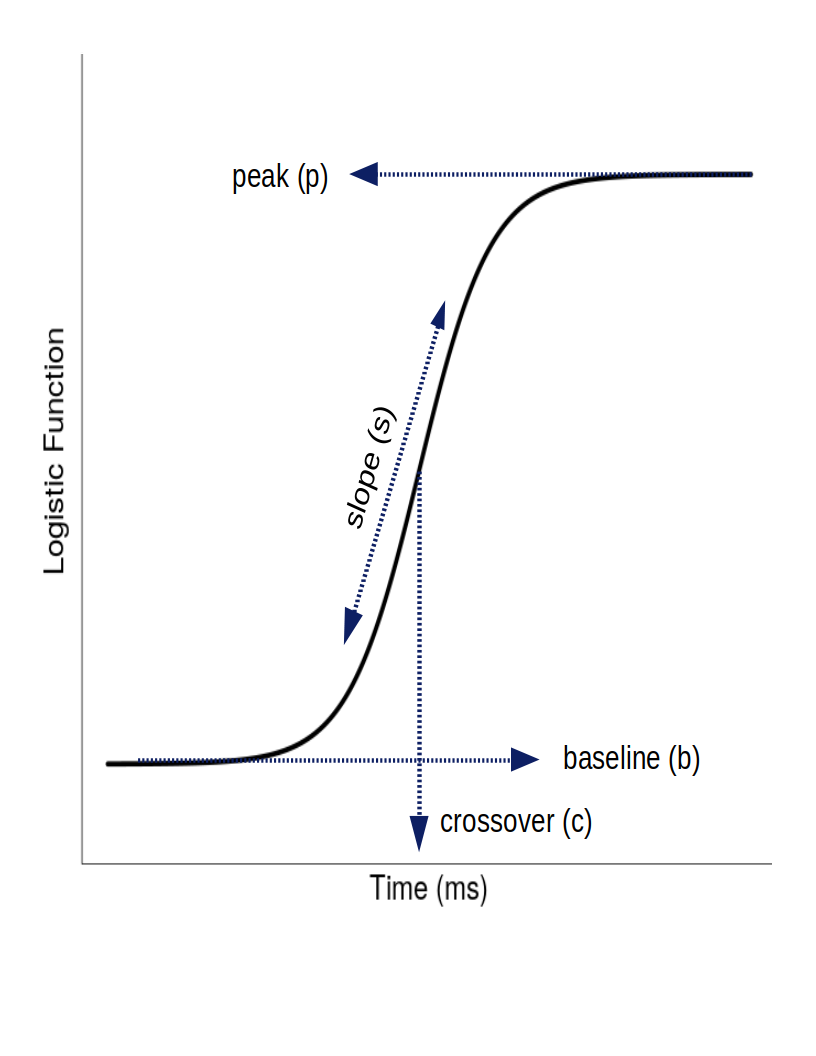
\includegraphics[scale=0.4]{logistic_label.png}
\caption{An illustration of the four-parameter logistic and its associated parameters, introduced as a parametric function for fixations to target objects in McMurray 2010. Can describe the parameters in detail, but should also have the formula itself somewhere to be referenced. (Equation~\ref{eq:logistic})}
\label{fig:logistic_definition}
\end{figure}



\section{Analysis with VWP Data}

The following section goes into more detail on the specifics


\subsection{Anatomy of Eye Mechanics \cn{[this section needs new name]}}

In the context of eye tracking data and word recognition, there are a few mechanics with which we are concerned. The first of these is activation. Even with the immediacy and (fullness? some word they use to describe dense time series here being better than yes/no response), what we observe with any eye movement is not a direct readout of the underlying activation.  Rather, there is a period of latency between the decision to launch an eye movement and the physiological response, a period known as oculomotor delay. And finally, there are they physical mechanics of the eye movements themselves, the saccade and the fixation which, together, make up a ``look". We will briefly address each of these in the reverse of the order in which they were introduced.



\paragraph{Saccades and fixations:} Rather than acting in a continuous sweeping motion as our perceived vision might suggest, our eyes themselves move about in a series of short, ballistic movements, followed by brief periods of stagnation. These periods of movement and stagnation, respectively, are the saccades and fixations. 

Saccades are short, ballistic movements lasting between 20ms-60ms, during which time we are effectively blind. Once in motion, saccades are unable to change trajectory from their intended destination. Following this movement is a period known as a fixation, itself made up of a necessary refraction period (during which time the eye is incapable of movement) followed by a period of voluntary fixation which may include planning time for deciding the destination of the next eye movement; the duration of fixations are typically (some length). It will be convenient to follow previous convention and consider a saccade followed by its adjacent fixation as a single concept called a ``look" \cite{mcmurray2002look}. We take particular care here to note that the beginning of a look, or ``look onset", starts the instance that a previous look ends or, said another way, the instant an eye movement is launched. A visual description of these is provided in Figure~\ref{fig:sac_fix_look}.



\begin{figure}[H]
\centering
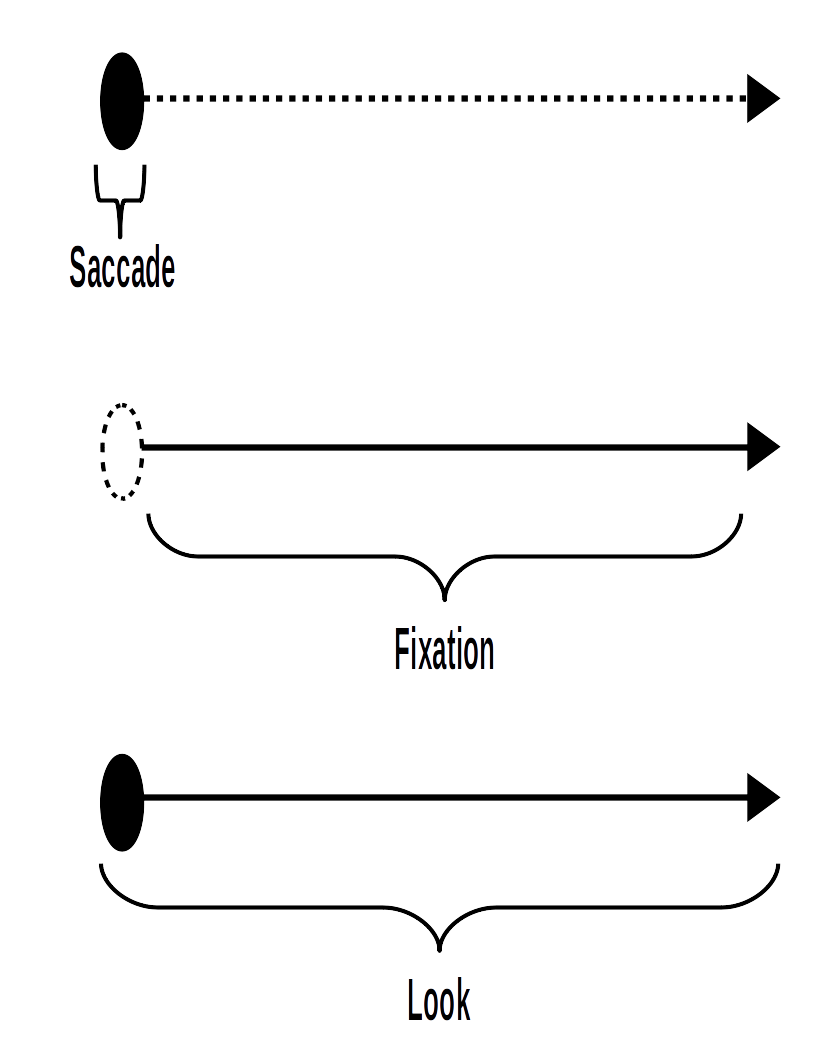
\includegraphics[scale=0.25]{sac_fix_look.png}
\caption{redo this image to match anataomy of look image, also for size}
\label{fig:sac_fix_look}
\end{figure}

\paragraph{Oculomotor delay:} While the physiological responses are what we can measure, they are not themselves what we are interested in. Rather, we are interested in determining word activation, itself governing the cognitive mechanism facilitating movements in the eye. Between the decision to launch an eye movement (a cognitive mechanism governed by the activation, next section) and the movement itself is a period known as oculmotor delay. It is typically estimated to take around 200ms to plan and launch an eye movement \cite{viviani1990time}, and this is usually accounted for by subtracting 200ms from any observed behavior. As oculomotor delay is only ``roughly" estimated to be around 200ms, we suggest that accounting for randomness will be critical in correctly recovering the the cognitive mechanism of interest or at very least in identifying possible sources of bias or error. How this phenomenon relates to saccades and fixations is demonstrated in Figure~\ref{fig:sac_fix_look_om}.


\begin{figure}[H]
\centering
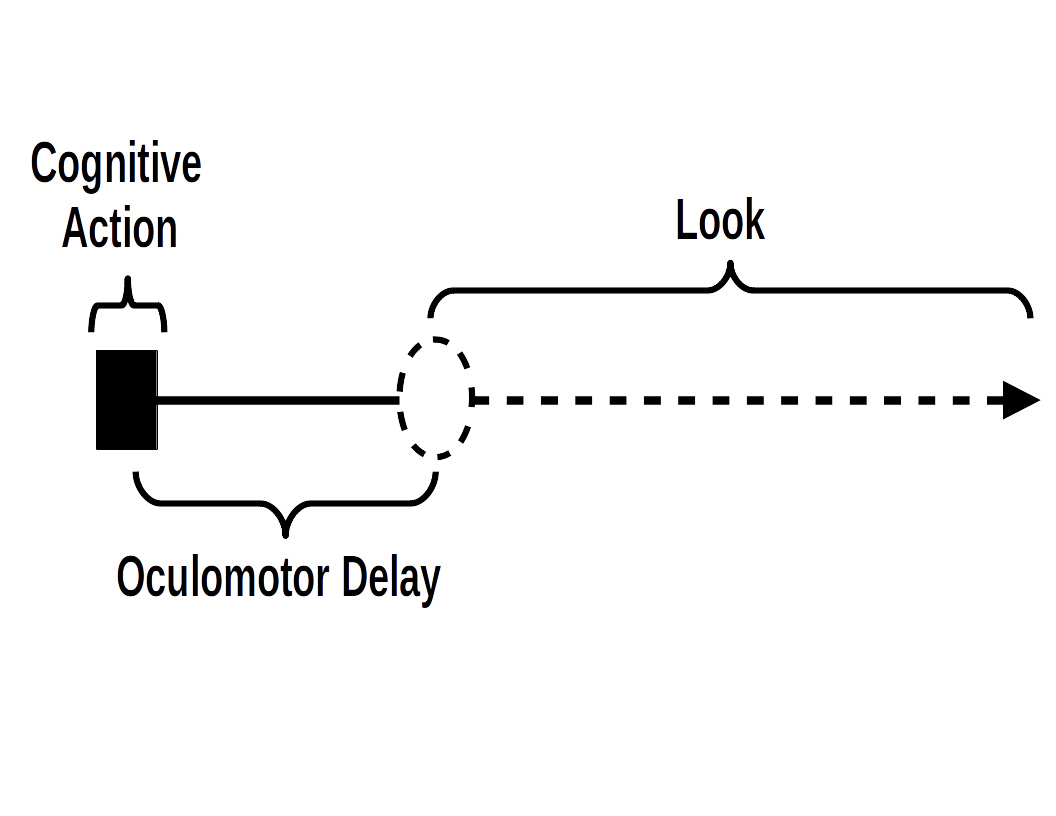
\includegraphics[scale=0.25]{om_delay2.png}
\caption{redo this image}
\label{fig:sac_fix_look_om}
\end{figure}


\begin{figure}
\centering
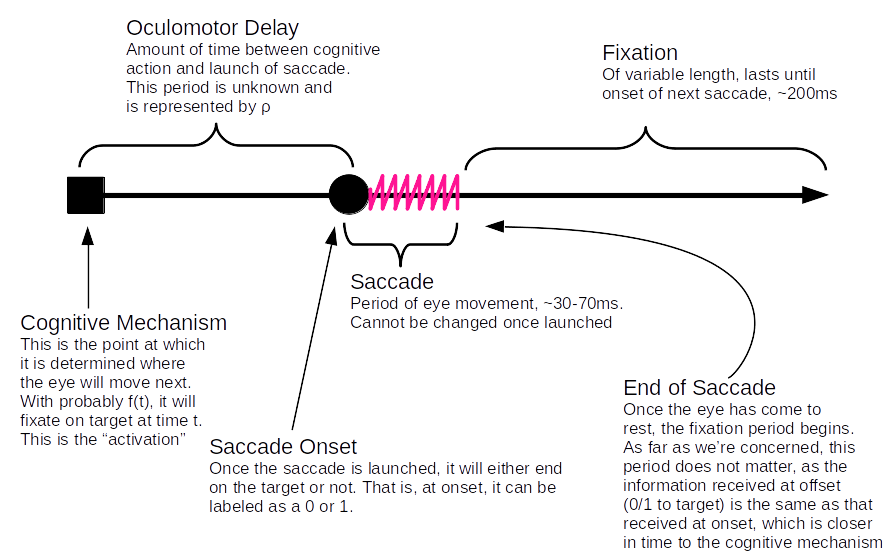
\includegraphics[scale=0.5]{labeled_full_diagram.png}
\caption{I want to do this figure again but differently. have saccade be  two bars matching anatomy of look, include refractory period of fixation, noting that that and saccade are identical, followed by period of time of voluntary fixation (theoretically relevant) followed by next CM}
\label{fig:full_diagram_looks}
\end{figure}

\begin{figure}
\centering
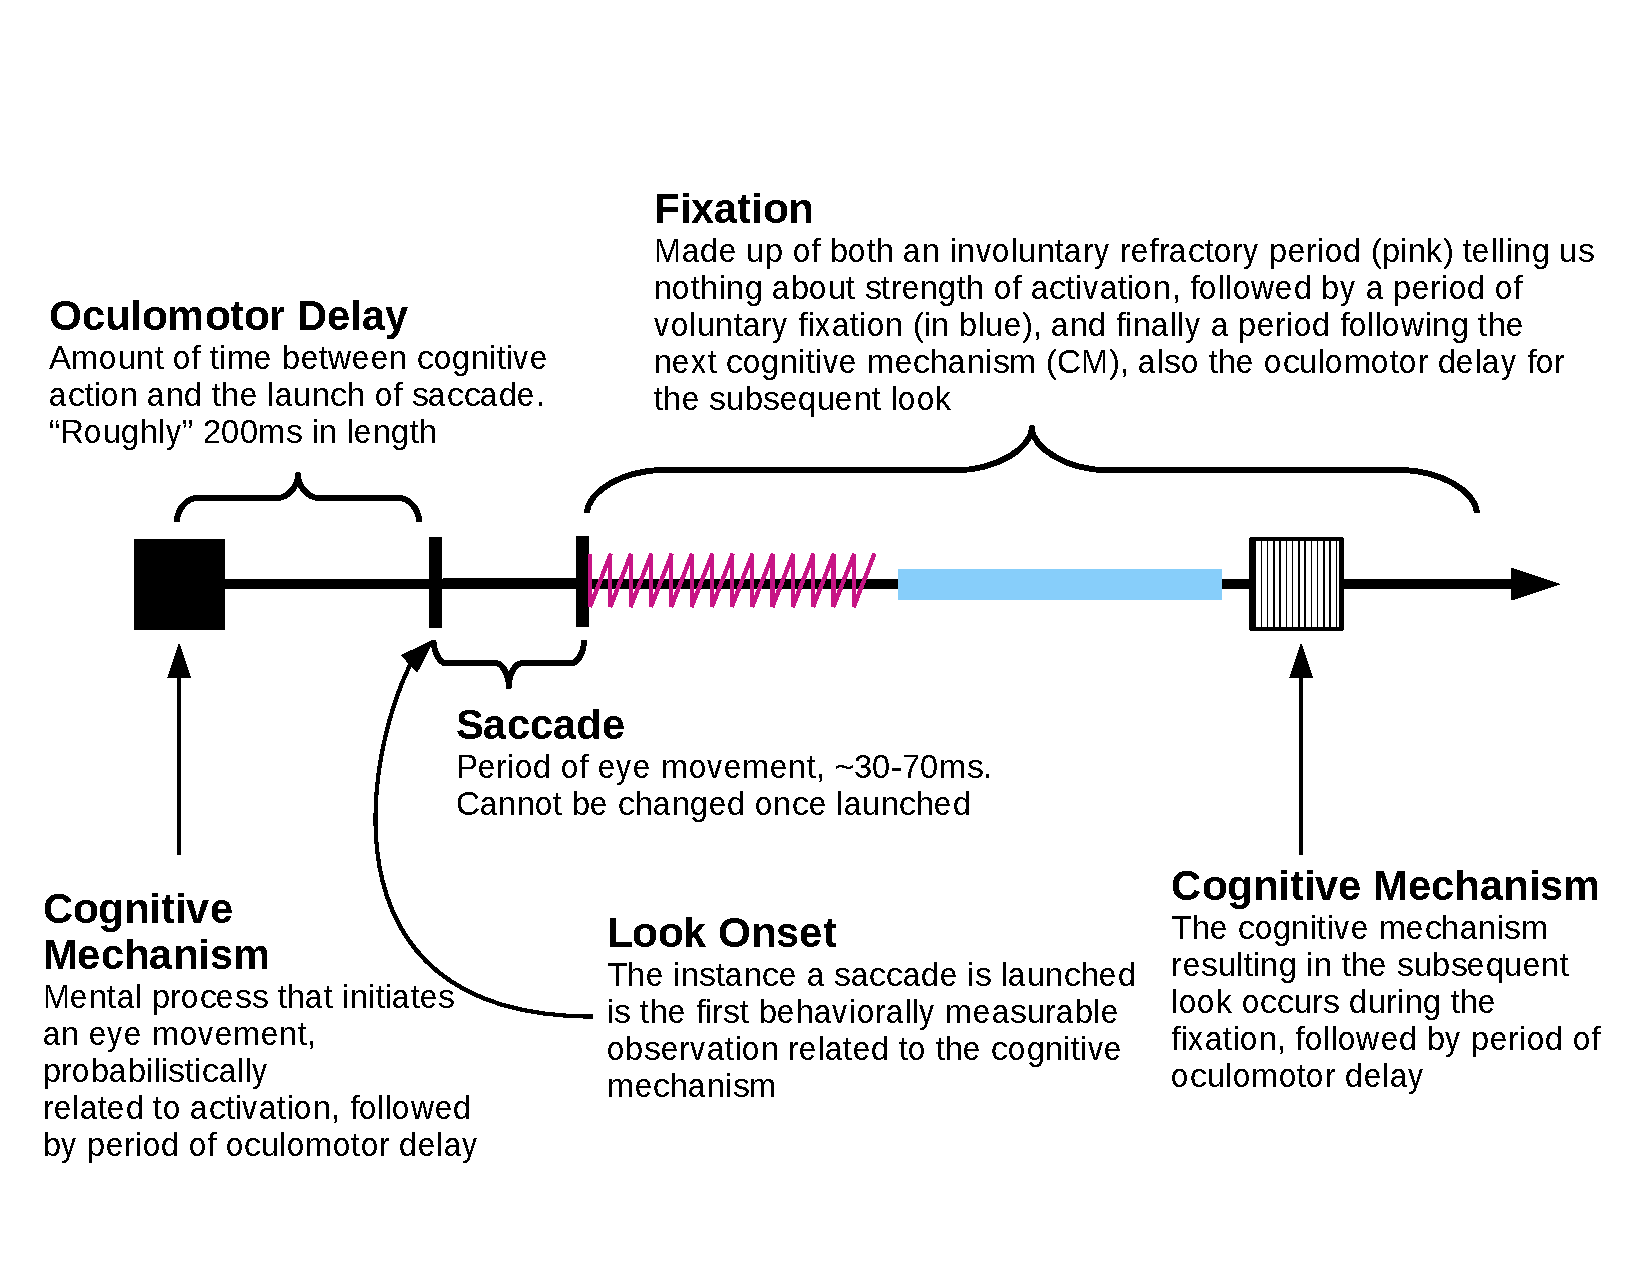
\includegraphics[scale=0.5]{what_is_a_look.pdf}
\caption{Alternative to Figure~\ref{fig:full_diagram_looks} with diagram of saccade/fixation more consistent with Figure~\ref{fig:anatomy_of_look}. There may be a bit more than is needed here, especially with the pink and blue (and maybe even subsequent CM). Although I don't discuss their use in detail, the pink/blue/second CM highlight the fact that \textit{even when} we argue that using proportion of fixation method indirectly captures strength of activation via length of duration, the assumption of linearity is incorrect. For the sake of argument, assuming that the refractory period is exactly 100ms and the length of oculomotor delay is 200ms, a fixation of length 500ms may seem to be 25\% larger than a fixation lasting 400ms, but in terms of the \textit{intentional} fixation period, it is twice as large. This serves both to demonstrate another issue with the proportion method while also paving the way for incorporating fixation length in the future. Still, this may not all be necessary here, or presented in a cleaner way} 
\label{fig:whats_in_a_look}
\end{figure}

\subsection{Activation}

The concept of activation, as it relates to the discussion here, arises from the metaphor in which word perception is made up of a network made up of hierarchical levels (letter, phoneme, word, etc.,) acting as an interactive process unfolding in time \cite{McClelland1981}. Under this \textit{interactive activation model}, greater activation is associated with a greater excitatory action for a network node (specifically here, a word) resulting from consistency with the received auditory signal. The interactive activation model allows for both excitatory and inhibiting activations, resulting in the ``competing" activation curves being modeled in the VWP. [maybe also address happens continuously, hence the continuous mapping model of lexical activation]

Here tie in idea of activation, though need to be more concise about what we mean. \cn{Good source for framework being (McClelland and Rumelhard 1981? Rumelhart and McClelland 81 and 82, and mcclelland/elman 86 with trace). They seem to all mention the ``interactive activation framework" which may be worthwhile to elaborate on further. For now, assume that we have adequately stated \textit{what it is}.}

While a number of experimental methods are used as real-time indices of lexical access (\cite{Spivey2005}, others), we concern ourselves here with the use of eyetracking as it relates to activation as first suggested by \cite{allopenna1998tracking}. Whereas the initial treatment of eyetracking data made no attempt identify or model subject-specific trends, more recent work has made strides in making subject analysis more tractable. Specifically, we adopt the idea that each participant's results can be fit to non-linear functions who's parameters describe clinically relevant properties \cite{mcmurray2010individual}. We will denote this activation function $f$ with parameters $\theta$ as a function in time, giving $f(t|\theta)$

For example, the four parameter logistic function in Figure~\ref{fig:logistic_definition} is often used to model fixations to the Target object in the VWP with functional form

\begin{equation} \label{eq:logistic}
f(t|\theta) = \frac{p-b}{1 + \exp \left(\frac{4s}{\text{p}-b} (x - t) \right)} + b.
\end{equation}

Similarly, a six parameter asymmetric Gaussian function, often used for fixations to competitors, is given as

\begin{equation} \label{eq:dg}
f(t|\theta) = \begin{cases}
\exp \left( \frac{(t - \mu)^2}{-2\sigma_1^2} \right) (p - b_1) + b_1 \quad \text{if } t \leq \mu \\
\exp \left( \frac{(t - \mu)^2}{-2\sigma_2^2} \right) (p - b_2) + b_2 \quad \text{if } t > \mu
\end{cases}
\end{equation}

(I didn't make a nice graph/label for this). 

While both functions are commonly used in the VWP for modeling eye fixations, for simplicity we will limit the primary focus of our discussion to fixations to the Target with the four parameter logistic, though ultimately our argument is agnostic to the modeling function used, parametric or otherwise. Discussion related to the asymmetric Gaussian is treated in the appendix.


\subsection{VWP data}


We now consider how the aforementioned mechanics relate to the visual world paradigm. In a typical instantiation of the VWP, a participant is asked to complete a series of trials, during each of which they are presented with a number of competing images on screen (typically four). A verbal cue is given, and the participants are asked to select the image corresponding to the spoken word. All the while, participants are wearing (generally) a head-mounted eye tracking system recording where on screen they were fixated. 

An individual trial of the VWP may be short, lasting anywhere from 1000ms to 2500ms before the correct image is selected. Prior to selecting the correct image, the participant's eyes scan the environment, considering images as potential candidates to the spoken word. As this process unfolds, a snapshot of the eye is taken at a series of discrete steps (typically every 4ms) indicating where on the screen the participant is fixated. A single trial of the VWP typically contains no more than four to eight total ``looks" before the correct image is clicked, resulting in a paucity of data in any given trial.

[relevant quote][``We find that eye movements to objects in the workspace are closely time-locked to referring expression s in the unfolding speech stream, providing a sensitive and nondistruptive measure of spoken language comprehension during continuous speech" \cite{allopenna1998tracking}]

To be clear, eye trackers themselves only record $x$ and $y$ coordinates of the eye at any given time, and it is only after the fact that ``psychophysical" attributes are mapped onto the data (saccades, fixations, blinks, etc.,). We adopt the strategy of prior work in discussing eye tracking data in terms of their physiological mapping, as this will be crucial in constructing a physiologically relevant understanding of the problem at hand \cite{mcmurray2002look}.

[``Default interpretation is that greater fixation proportions indicate greater activation in the underlying processing system" \cite{Magnuson2019}]


To create a visual summary of this process aggregated over all of the trials, a la Allopena, a ``proportion of fixations" curve is created, aggregating at each discrete time point the average of indicators of whether or not a participant is fixated on a particular image. A resulting curve is created for each of the competing categories (target, cohort, rhyme, unrelated), creating an empirical estimate of the activation curve, $f(t|\theta)$. See Figure~\ref{fig:bob_diagram_full}. For any subject $i = 1, \dots, n$, across times $t = 0, \dots, T$ and trials $j = 1, \dots, J$, a construction  of this curves can be expressed as:


\begin{equation}\label{eq:sum_proportions}
y_{it} = \frac1J \sum z_{ijt}
\end{equation}
where $z_{ijt}$ is an indicator $\{0, 1\}$  towards a particular object in trial $j$ at time $t$ and such that we have an empirical estimate of the activation curve,
\begin{equation}\label{eq:empir_to_activation}
f(t | \theta_i) \equiv y_{it}.
\end{equation}



For our discussions here, we will call this the proportion of fixation method (though we not that in actuality it is the proportion of \textit{trials} in which a fixation occurs at each time point).


\begin{figure}[H]
\centering
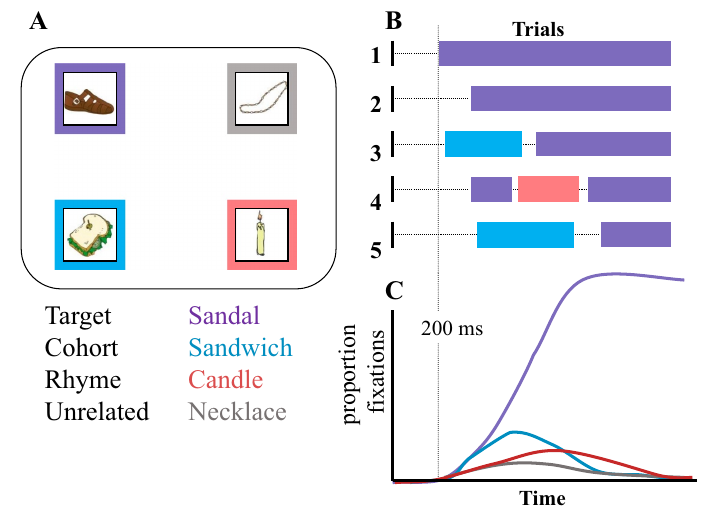
\includegraphics[scale=0.45]{bob_vwp_full.png}
\caption{Stole this from Bob (who apparently stole it from richard aslin), plan on making my own}
\label{fig:bob_diagram_full}
\end{figure}

\begin{figure}[H]
\centering
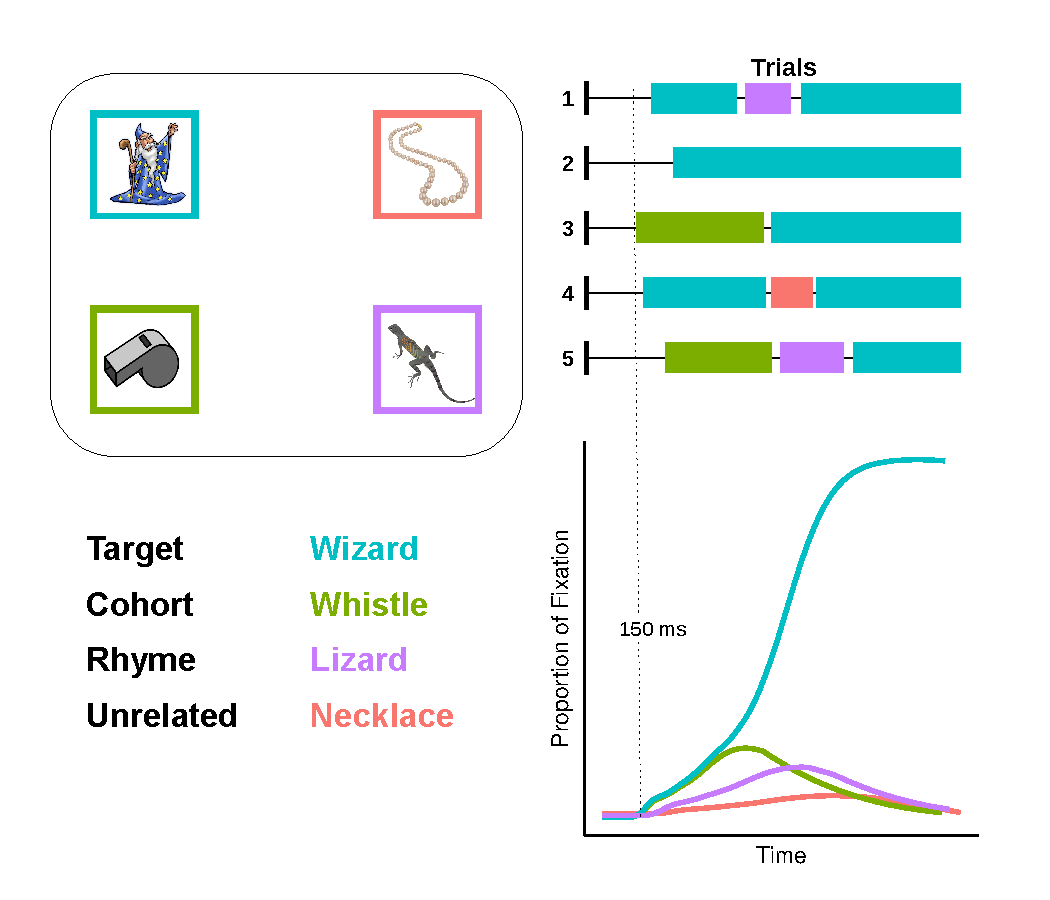
\includegraphics[scale=0.7]{collin_diagram_full.pdf}
\caption{Stole this from Bob (who apparently stole it from richard aslin), plan on making my own}
\label{fig:collin_diagram_full}
\end{figure}



As each individual trial is only made up of a few ballistic movements, the aggregation across trials allows for these otherwise discrete measurements to more closely represent a continuous curve. Curve fitting methods, such as those employed by \xt{bdots}, are then used to construct estimates of function parameters fitted to this curve. Figure~\ref{fig:bob_diagram_full} provides an illustration.


\section{Look Onset}

Though eye-tracking data is what we are able to observe, it itself is not what we are interested in; rather, it is the cognitive process directing eye movements and how it relates to underlying lexical activation. How the physiological response relate to this process is known as a \textit{linking hypothesis} \cite{Magnuson2019}. In the context of the Visual World Paradigm, the linking hypothesis is often only implicitly defined, with ``the default interpretation [seeming] to be that greater fixation proportions indicate greater activation in the underlying language processing system." 

The simplest version of a linking hypothesis given in this context is that of \cite{allopenna1998tracking}, with  the ``general assumption that the probability of initiating an eye movement to fixate on a target object $o$ at time $t$ is a direct function of the probability that $o$ is the target given the speech input and where the probability of fixating $o$ is determined by the activation level of its lexical entry relative to the activations of other potential targets (i.e., the other visible objects)." To a degree, this assumption is shared by most linking hypotheses in that the probabilistic nature of the proportions of fixations is assumed to be related in time to the strength of the underlying activation. Primary differences in linking hypotheses tend to revolve around the particulars of the mechanics involved, including the duration of fixations, eye scanning behavior, the impacts of priming, or the relation between visual  processing acting in conjunction with lexical activation. We make no statement as to the merits of each, though see \cite{Magnuson2019} for a review.

A more recent review probed the relationship between the observed dynamics and underlying activation in the context of attempting to recover the latter from the former \cite{mcmurray2022m}. This was done through a series of simulations in which fixations were constructed sequentially with a collection of sampling and generating procedures. In short, this contribution showed that curves reconstructed using the standard proportion of fixations method were poor estimates of the underlying system, with the magnitude of bias in estimation increasing with the complexity of the mechanisms involved.

An important contribution made there, however, was the explicit definition of the underlying activation function. Though consistent with the equivalence often assumed in Equation~\ref{eq:empir_to_activation}, it is marked in that [it positively specified activation to be recovered rather than positively specifying a function to fit the observed data from which we then make statements about activation. I'm not saying this well]

From this, and in light of the relationship between the the cognitive process and the eye mechanics presented in Figure~\ref{fig:whats_in_a_look}, there is a fundamental problem with the equivalence suggested in Equation~\ref{eq:empir_to_activation}, arising from the fact that the decision to launch an eye movement is made up of a fundamentally distinct (though related) mechanism than that which determines the duration of fixation. Specifically, if we assume that the cognitive mechanism responsible for \textit{initiating} an eye movement is probabilistically related to activation, then we argue that using \textit{only} the instance of a look onset (beginning with the initiation of a saccade) is a more theoretically consistent and physiologically defensible observation to treat as relevant data.[ We will save discussion on treatment of the rest of the fixation data for later.]


We propose here what we call the \textit{look onset method}, which holds that the destination of a saccade launched at time $t$, $s_t$, is probabilistically determined by its lexical activation at time $t$. Letting $f(t|\theta)$ denote the lexical activation to the Target at time $t$, for example, gives

\begin{equation}\label{eq:onset_distribution}
s_t \sim Bern \big[ f( t  |  \theta) \big].
\end{equation}

In other words, we argue that the destination of a look is probabilistically determined by the cognitive mechanism demonstrated in Figure~\ref{fig:whats_in_a_look} as a function of activation. In reference to an object $o$, the decision to initiate a look to that object is inherently a Bernoulli event. Following a period of oculomotor delay, a saccade is launched and the destination of the saccade is the first instance in which we observe the outcome of the cognitive process in question. However, as the destination of a saccade cannot change once launched, this outcome is already determined at saccade onset, making the onset the earliest instance in which see evidence of the cognitive mechanism, even if its outcome is not known until the saccade has finished. By marking this onset as the only relevant data, we limit our observed data to follow the same distribution as the process in question. By instead including the entire duration of a fixation, one introduces what we call \textit{added observation bias}.

By added observation bias, I am referring to the fact that in a standard analysis of the VWP using the proportion of fixation method, the entire duration of a fixation is indicated with a $\{0,1\}$ at any time $t$, without having observed any additional behavior associated with the cognitive mechanism responsible for initiating an eye movement at that time. By using the entire fixation, we are both obscuring data that is relevant to the mechanism of interest (onset) while also conflating it with data generated by a fundamentally different process. If a look onset at time $t$ is probabilistically determined by its lexical activation $f(t|\theta)$, then treating the period of subsequent fixation as indistinguishable has the effect of not only ``adding" observations to the data, but adding observations that are inherently biased. The result is a distorted estimate of the underlying activation. A depiction of this phenomenon is given in Figure~\ref{fig:folly_of_fixation}.

\begin{figure}[H]
    \centering
    \subfigure[]{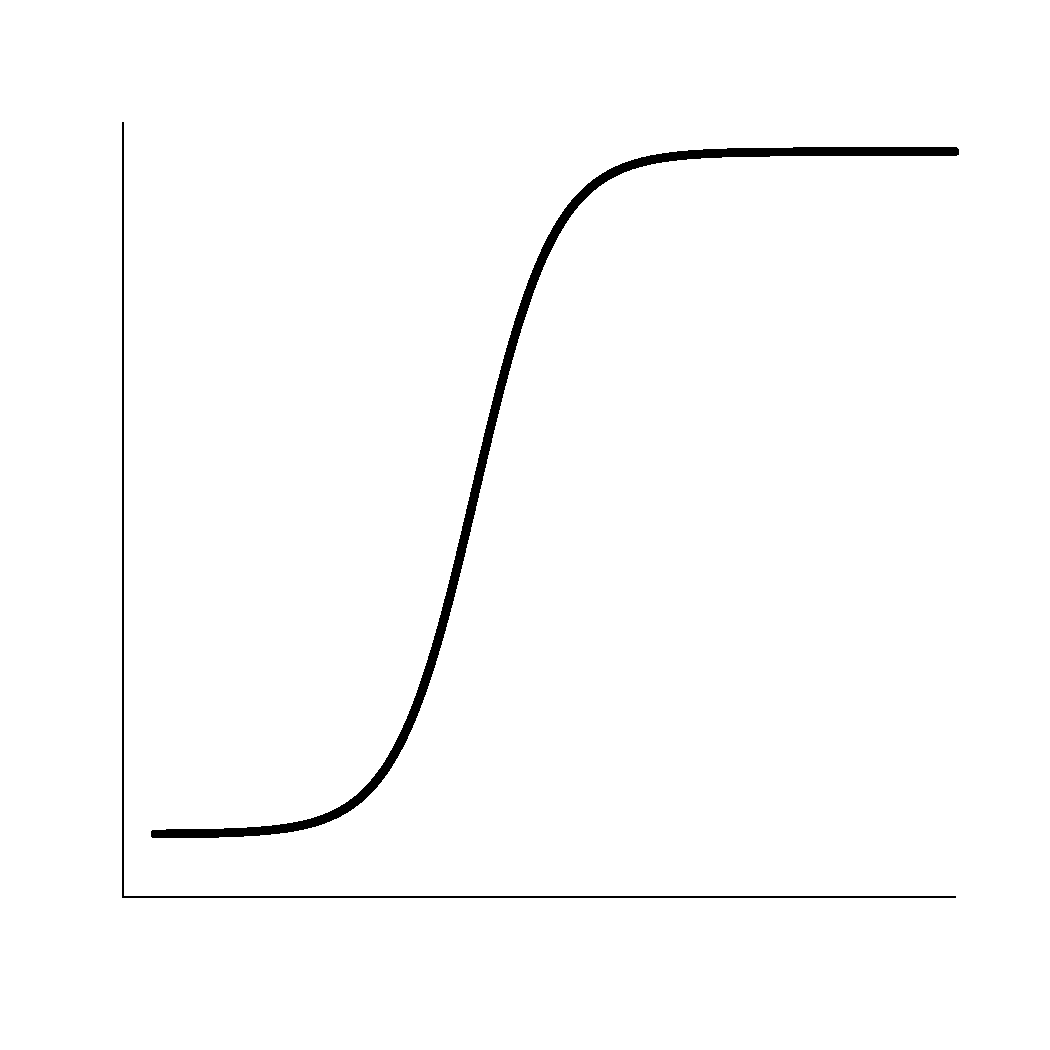
\includegraphics[width=0.45\textwidth]{logistic_a.pdf}} 
    \subfigure[]{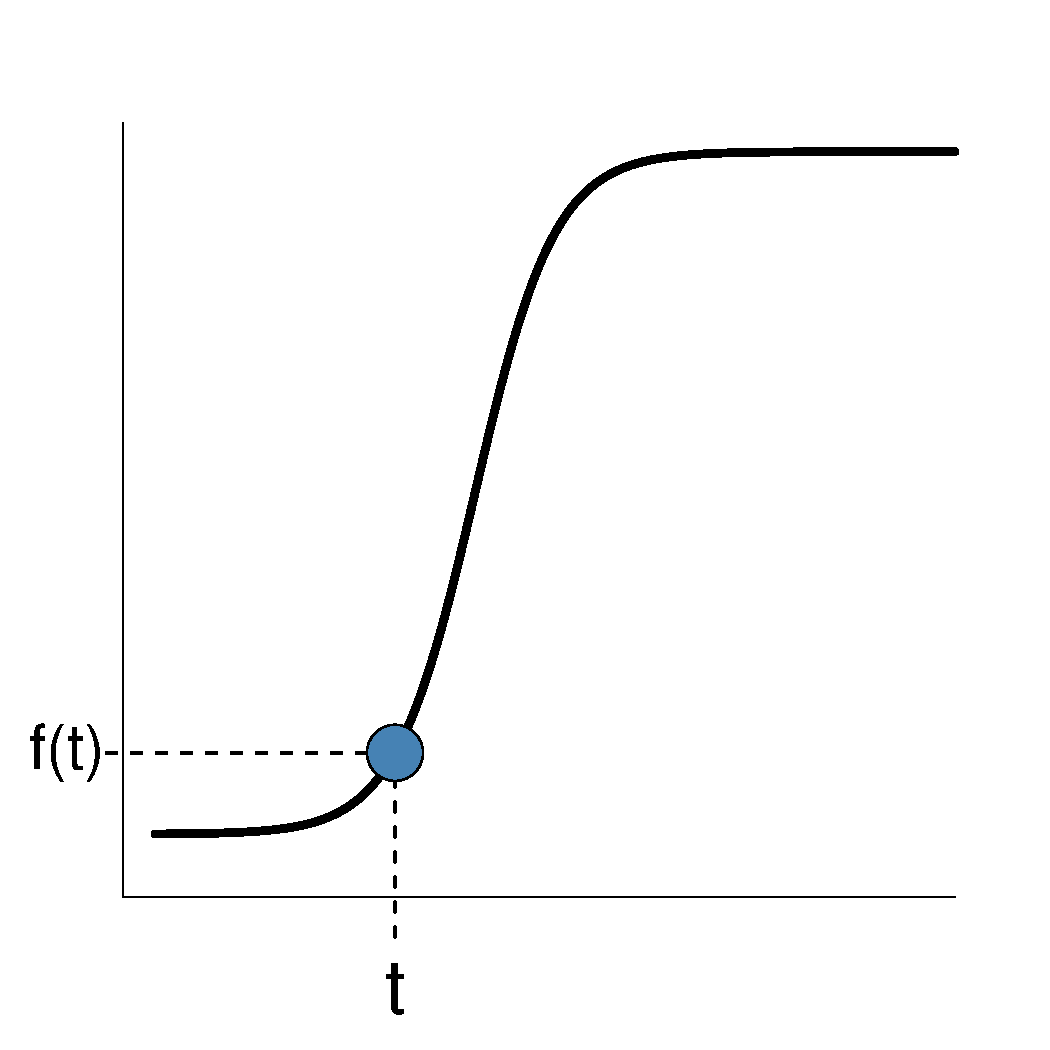
\includegraphics[width=0.45\textwidth]{logistic_b.pdf}} 
    \subfigure[]{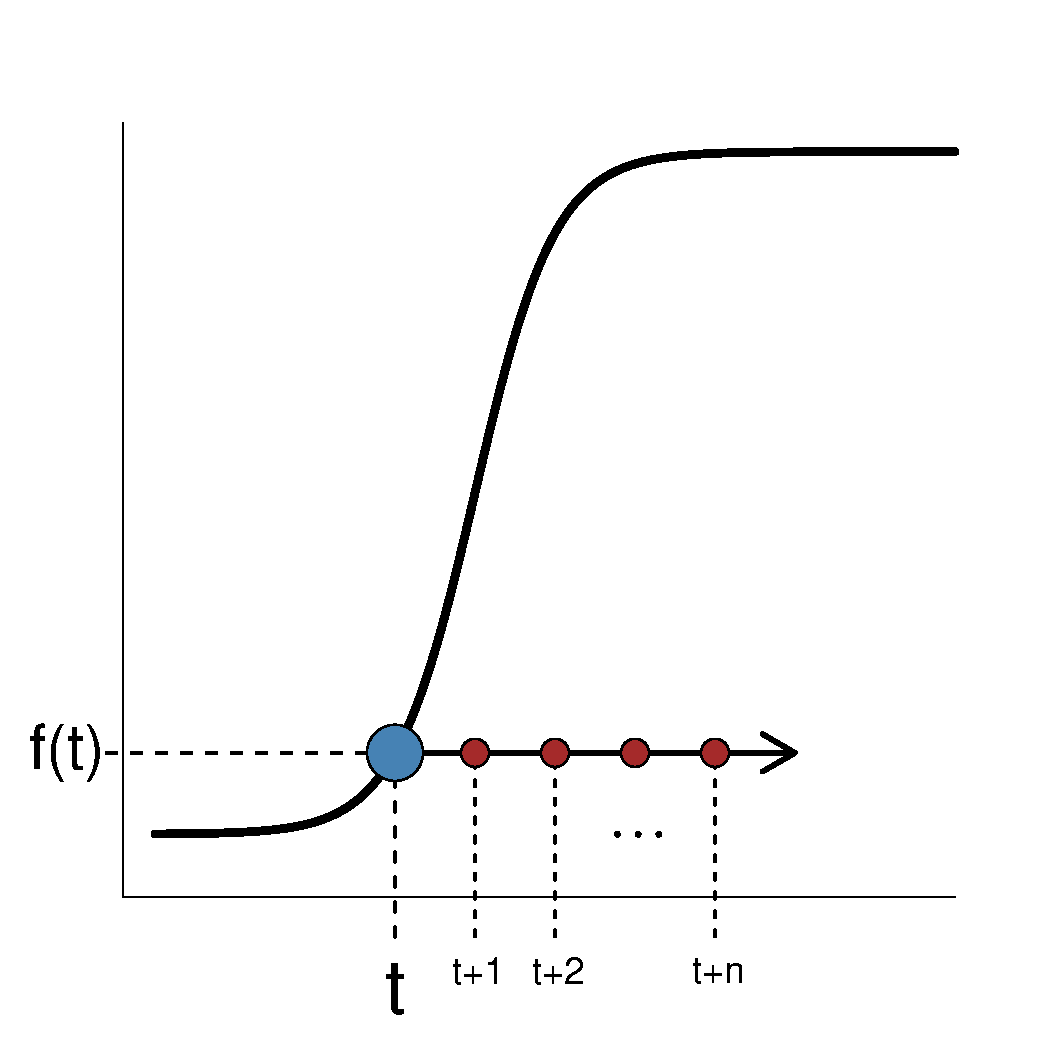
\includegraphics[width=0.45\textwidth]{logistic_c.pdf}}
    \caption{ \textbf{(a.)} Example of a nonlinear activation curve $f(t|\theta)$ \textbf{(b.)} At some time, $t$, a saccade is launched with its destination probabilistically determined by $f(t|\theta)$ \textbf{(c.)} For a look persisting over $n$ time points, $t+1, \dots, t+n$, we are recording ``observed" data, adding to the proportion of fixations at each time but without having gathered any additional observed data at $f(t+1 | \theta), \dots,f(t+n | \theta)$, thus inflating (or in the case of a monotonically increasing function like the logistic, deflating) the true probability. }
\label{fig:folly_of_fixation}
\end{figure}

To be clear, this is not to say that the length of a fixation has no relevant information regarding the strength of activation, and indeed numerous studies (source?) have demonstrated this to be the case. Rather, we argue that by more clearly specifying the particular process that we are interested in, we can perform better recovery of the underlying mechanism. (don't like this sentence).

[not sure if i need paragraphs or subsections, but kind of a break here to next topic and something else we investigate in the simulations]

Because of oculomotor delay, which we define as $\rho$, a look onset observed at time $t$ is not actually determined with probability $f(t|\theta)$ but rather $f(t - \rho|\theta)$. As mentioned previously, this delay is typically acknowledged to be ``roughly" 200ms, and in a standard analysis it is usually accounted for with a horizontal shift of 200ms to the observed data. The ability to correctly specify and correct for this delay is critical, particularly in situations such as the look onset method in which the total data is much sparser and potentially much more sensitive to misspecification. 

There are two qualities of oculomotor delay that we consider here. The first is the simple observation that any difference between the true mean duration of oculomotor delay and the 200ms adjustment will result in bias. Second, we observe that in the case in which the mean duration of oculomotor delay is 200ms (and there is no bias present), the degree of randomness will have a direct effect on the observed error in the recovery of the underlying activation function. And while we don't provide any specific solutions to this problem yet, by highlighting the potential impact in simulation we demonstrate a need for further investigation.




%
%
%\section{Bias/Look Onset (better name for section)} 
%
%
%Having given due consideration to the state of things are they are, we find ourselves in a time of moral reflection, reexamining the underlying relationship between lexical activation (the mechanism of interest) and the physiological behavior we are able to observe (here, specifically eye-tracking). This is referred to in the literature as the linking hypothesis. And while there are a number of competing hypothesis, they each share a collection of implicit assumptions relating what is observed to what is being studied.
%
%The simplest version of a linking hypothesis in the context of the VWP is the ``general assumption that the probability of initiating an eye movement to fixate on a target object $o$ at time $t$ is a direct function of the probability that $o$ is the target given the speech input and where the probability of fixating $o$ is determined by the activation level of its lexical entry relative to the activations of other potential targets (i.e., the other visible objects)" \cite{allopenna1998tracking}. It is from this assumption that we justify the relation in Equation~\ref{eq:empir_to_activation}. To a degree, this assumption is shared by most linking hypothesis in that the probabilistic nature of the proportions of fixations is assumed to be related in time to the strength of the underlying activation. Primary differences in linking hypotheses tend to revolve around the particulars of the mechanics involved, including the duration of fixations, eye scanning behavior, the impacts of priming, or the relation between visual  processing acting in conjunction with lexical activation. We make no statement as to the merits of each, though see \cite{Magnuson2019} for a review.
%
%We consider a particular meta contribution to this debate presented by McMurray in which he probed the relationship between the observed dynamics in the fixations and the underlying dynamics of activation under a variety of assumptions \cite{mcmurray2022m}. In short, he showed that curves reconstructed using the standard proportion of fixations analysis in the VWP were poor estimates of the underlying system, with the magnitude of bias increasing with the complexity of the mechanisms involved. Though this made few claims as to what the underlying mechanics may be, it did demonstrate the inherent difficulty in relating observable behavior to the underlying cognitive process.
%
%An important contribution made there, however, and one that we adopt here is an explicit definition of the underlying activation function. Given the relation in Equation~\ref{eq:empir_to_activation}, it is reasonable to assume that the underlying activation of any of the objects with the VWP could be modeled with a nonlinear function $f(t|\theta)$. The goal of a VWP analysis, then, is the recovery of this underlying activation function.
%
%From this assumption we propose an alternative model of the relation between the underlying activation and the observed behavior, with a careful delineation of the psycho-physical components of a look in conjunction with its generating behavior. In particular, we consider the cognitive mechanism associated with initiating an eye movement, which is probabilistically associated with lexical activation, the delay between this and the onset of its associated look, and finally how the different components of the look are related to fundamentally different mechanisms. From this and what we ultimately argue is that observed bias in the recovery of the activation curve under the proportion of fixations method can be partitioned into two distinct components:
%
%[i would like to maybe go into more detail here or have a picture]
%
%%\begin{singlespace}
%\begin{enumerate}
%\item The first source of bias, which is the primary emphasis of my proposal, is what I call the ``added observation" bias. This involves the fact that in  a standard analysis of VWP data, the entire duration of a fixation is indicated with a $\{0,1\}$  at any time, $t$, without having observed any behavior associated with the initiation of an eye movement at that time. In other words, by using the entire fixation, we are both obscuring data relevant to the mechanism of interest (onset) while also conflating it with data generated by a fundamentally different mechanism [unpack this a bit more here].
%\item The second source of bias is ``delayed observation bias". This bias arises from the fact that an eye movement launched at some time $t$ was planned at some time prior. This is primarily a consequence of the oculomotor delay
%\end{enumerate}
%%\end{singlespace}
%
%The first source of bias, the ``added observation" bias, arises singularly from the fact that the destination of a look, which is observed at look onset, has a fundamentally \textit{different} generating mechanism than what determines the duration of a look, never minding such mechanics as the duration of a saccade or the refractory period of a fixation. Nonetheless, a standard analysis of VWP data does not differentiate between the initial onset and the period of subsequent fixation: both are recorded as either $0$ or $1$ according to it's location. A look onset at time $t$ is probabilistically determined by by its lexical activation $f(t|\theta)$ whereas the period of fixation is governed by a separate mechanism altogether. Treating the subsequent fixation as indistinguishable has the effect of not only ``adding" observations to the data, but adding observations that necessarily biased. The result is a distorted estimation of the underlying activation. A depiction of this phenomenon is given in Figure~\ref{fig:folly_of_fixation}. 


%\begin{figure}[H]
%    \centering
%    \subfigure[]{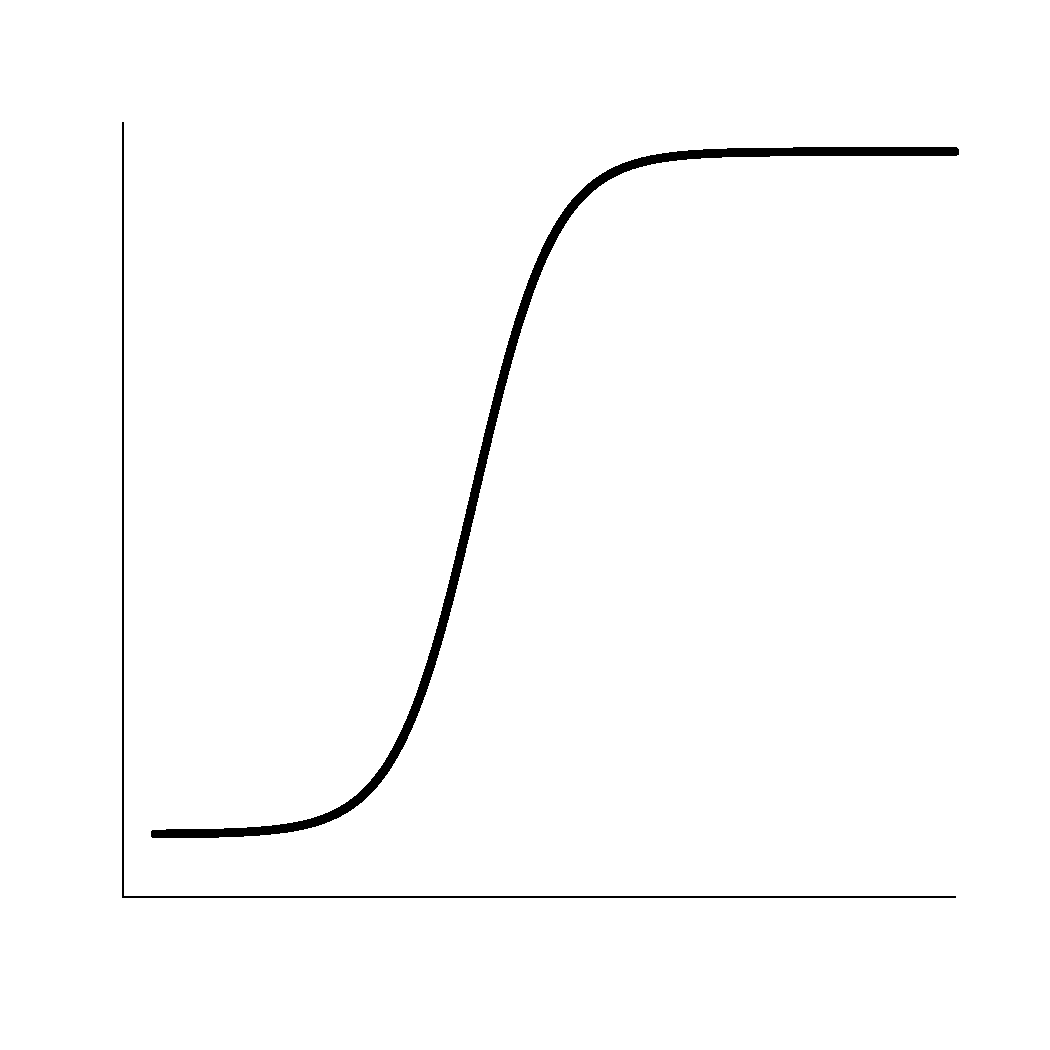
\includegraphics[width=0.45\textwidth]{logistic_a.pdf}} 
%    \subfigure[]{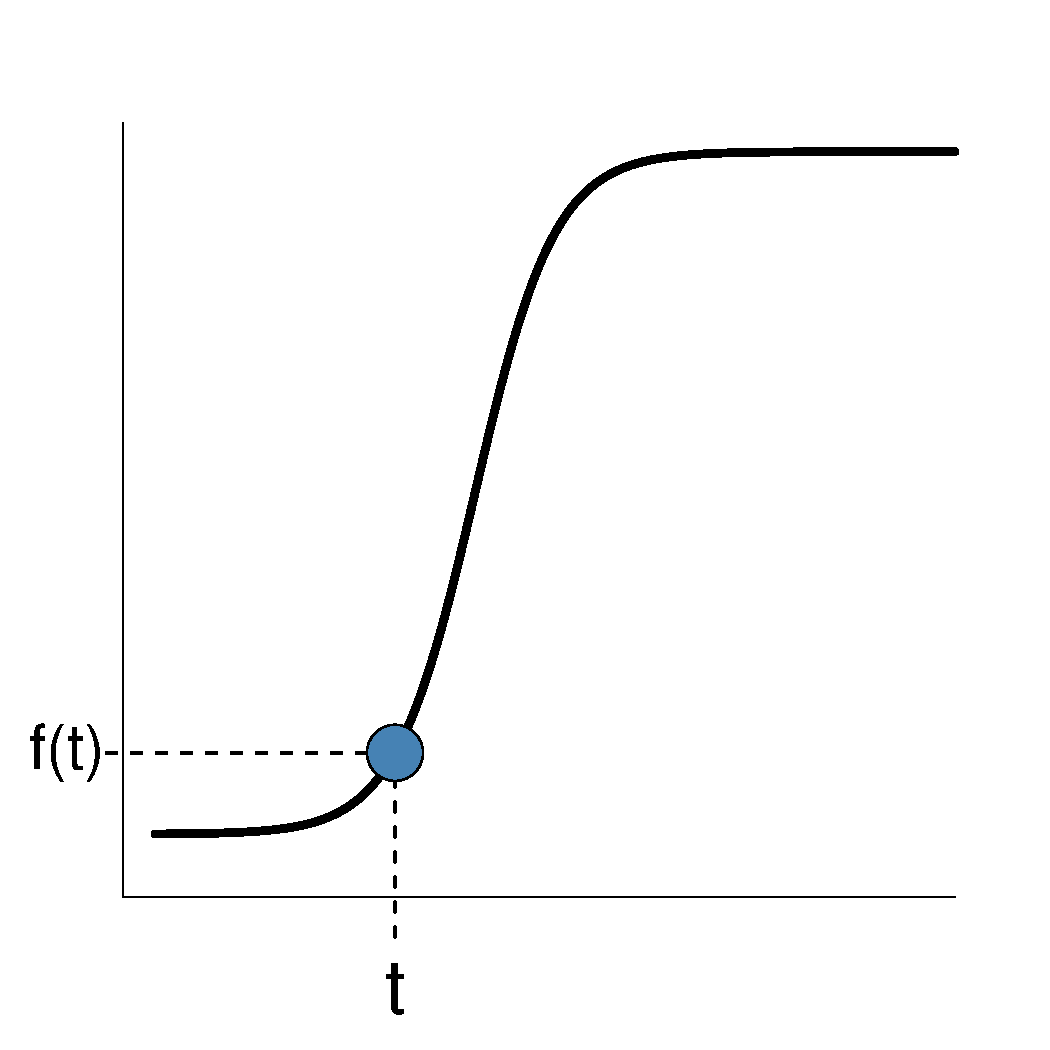
\includegraphics[width=0.45\textwidth]{logistic_b.pdf}} 
%    \subfigure[]{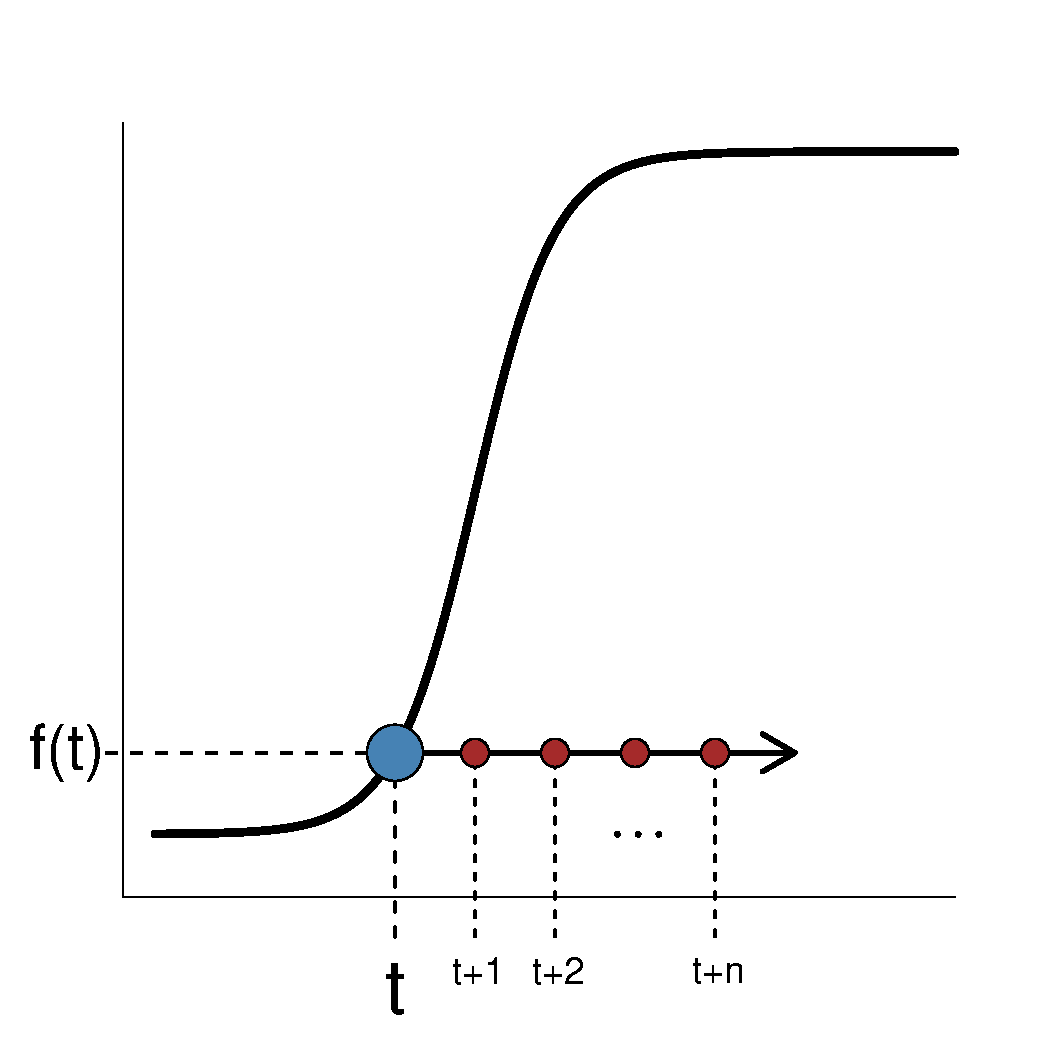
\includegraphics[width=0.45\textwidth]{logistic_c.pdf}}
%    \caption{ \textbf{(a.)} Example of a nonlinear activation curve $f(t|\theta)$ \textbf{(b.)} At some time, $t$, a saccade is launched with its destination probabilistically determined by $f(t|\theta)$ \textbf{(c.)} For a look persisting over $n$ time points, $t+1, \dots, t+n$, we are recording ``observed" data, adding to the proportion of fixations at each time but without having gathered any additional observed data at $f(t+1 | \theta), \dots,f(t+n | \theta)$, thus inflating (or in the case of a monotonically increasing function like the logistic, deflating) the true probability. }
%\label{fig:folly_of_fixation}
%\end{figure}

%The second source of bias is the ``delayed observation" bias. It is well established in the literature that the time it takes to plan and launch a saccade is around 200ms \cite{viviani1990time}, which is typically accounted for by subtracting 200ms from the observed data. There are two aspects of this that are worth considering further. First, if the mean duration of this oculomotor delay is not 200ms, bias will be observed as the difference between the true time and the 200ms adjustment. And although not bias in the technical sense, there has been no accounting for what effect randomness in this delay has on the error in the recovery of the underlying activation. It will be worthwhile in investigating this as the potential magnitude will determine if this delay is worth considering in any more detail in future research.
%
%---
%
%While we present no immediate solution to the effects of randomness in the delayed observation bias, we argue that the added observation bias can be rectified by using \textit{only} the times observed with look onset in the recovery of the underlying dynamics. We call this the the ``look onset" method, which we explain in more detail.
%
%We argue further that the added observation bias can be rectified by using \textit{only} the times observed with the look onset in the recovery of the underlying dynamics. We call this the ``look onset" method in contrast to the ``proportion of fixation" method. And while we do not present an immediate solution to the problem of the delayed observation bias, we do demonstrate the effects on estimation error in the presence of oculomotor delay even when the correct mean is accounted for.
%
%
%\paragraph{Look Onset Method:} The look onset method differ in the proportion of fixation method only in determining which observed data should be considered relevant in the estimation of lexical activation. A particularly compelling argument to made in favor of the look onset method, a corollary of the added observation bias, is that it has a readily defensible mathematical description. A saccade launched at time $t$ (marking the onset of a look) is assumed to be probabilistically determined by its lexical activation (relative to competitors) at time $t$, giving us
%
%\begin{equation} \label{eq:saccade_dist}
%s_t \sim Bin[f(t| \theta)]
%\end{equation}
%
%(it may be that $l_t$ for look onset is better notation, but my concern is that it doesn't capture the ``onset" nature that we are concerned with and may instead suggest the entire saccade + fixation).
%
%The utility of this is evident when tasked with stating the distribution of $y_t$ in Equation~\ref{eq:sum_proportions} as it relates to $f(t|\theta)$. And where given the overlap of fixations within a particular trial, it is unclear what relation $y_t$ may have to $y_{t+1}$. 
%
%[maybe statement along the lines of we make no assumptions as to the processing of visual stimuli, with probabilities of fixations independent of previous fixations? consistent with other ``bare bones" linking hypotheses]
%
%Two further comments are made about this method here. First, in anticipation of the observation that the look onset method discards relevant information regarding the strength of activation by not implicitly including the length of a fixation (source), we acknowledge this and reserve further comment for the discussion. Second, given the difference in structure of the observed data, we confirm that the current iteration of \xt{bdots} is capable of fitting nonlinear curves to data both under the proportion of fixation and look onset methods, removing any technical difficulties in the adoption of this method.


%
\section{Simulations}

In this section we construct a number of simulations to investigate the impact of added observation bias in the recovery of the underlying activation, as well as highlight the influence of randomness in the oculomotor delay in recovery. The simulations are constructed to emulate a typical study in the Visual World Paradigm, in which individual subjects are tasked with undergoing a series of trials, during each of which subjects make a series of fixations whose locations are probabilistically associated with lexical activation. For brevity, we consider in this section only those fixations associated with the Target object, modeled with the four parameter logistic as given in Equation~\ref{eq:logistic}; simulations according to looks to competitors is treated in the index, though the phenomenon we detail here are ultimately agnostic to any particular generating function. We will begin by detailing the process of simulating a single subject. 


\begin{figure}[H]
\centering
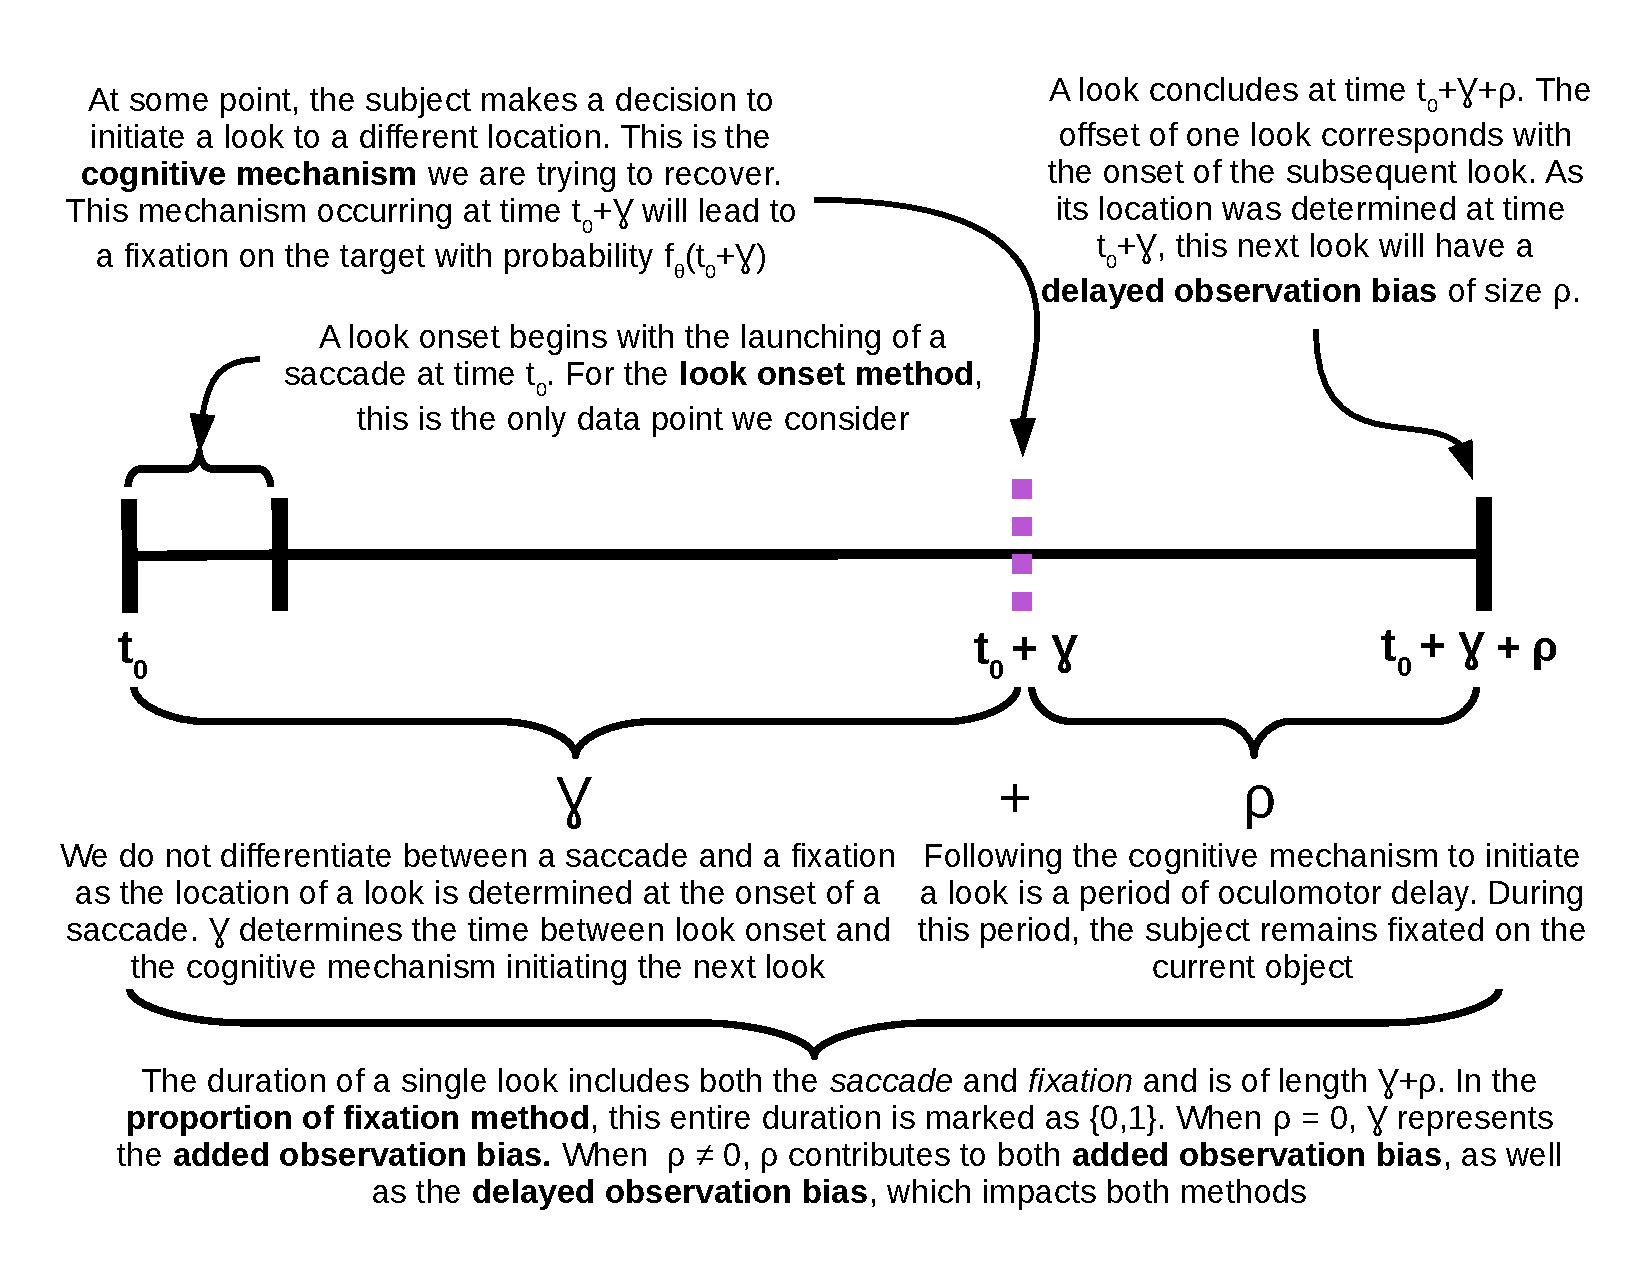
\includegraphics[width=\textwidth]{anatomy_of_look.pdf}
\caption{Anatomy of a look -- a key thing to discuss somewhere is the OM delay, refractory period, and planning time. The latter two go in $\gamma$. Worth noting also that while we do need to be able to control for $\rho$, \textit{information} regarding strength of consideration will be in $\gamma$ less the refractory period}
\label{fig:anatomy_of_look}
\end{figure}


First, each subject $i$ randomly draws a set of parameters $\theta_i$ from an empirically determined distribution based on normal hearing participants in the VWP \cite{FarrisTrimble2014} to construct a subject specific generating curve, $f(\cdot | \theta_i)$, where $f$ here is assumed to be the logistic given in Equation~\ref{eq:logistic}.   It is according to this function that the decision to initiate a look at time $t$ will subsequently direct itself to the Target with probability $f(t|\theta_i)$. We then go about simulating trials according to the following method: At some time $t_0$, a subject initiates a look. This look persists for at least a duration of $\gamma$, drawn from a gamma distribution with mean and standard deviation independent of time and previous fixations. At time $t_0+\gamma$, the subject determines the location of its next look, with the next look being directed towards the target with probability $f(t+\gamma | \theta_i)$. The decision to initiate a look is followed by a period of oculomotor delay, $\rho$, during which time the subject remains fixated in the current location. Finally, at time $t_0 + \gamma + \rho$, the subject ends the look initiated at $t_0$ and immediately begins its next look to the location determined at time $t_0 + \gamma$. For the look onset method, the only data recorded are the times of a look onset and their location: in this case, at times $t_0$ and $t_0 + \gamma + \rho$. By contrast, the proportion of fixation method records the object of fixation at 4ms intervals for the entire period of length $\gamma + \rho$. A single trial begins at $t = 0$ and continues constructing looks as described until the total duration of looks exceeds 2000ms. Each subject undergoes 300 trials, and 1,000 subjects are included in each simulation.

Three total simulations were performed to investigate the biases identified in the previous section, each differing only in the random distribution of the oculomotor delay parameter, $\rho$. In the first simulation, we set $\rho = 0$ to remove any oculomotor delay. In this scenario, a look initiated at time $t$ by subject $i$ will be directed towards the target with probability $f(t|\theta_i)$. Doing so removes any potential bias from delayed observation and allows us to identify the effects of the added observation bias in isolation. In the remaining simulations we probe the effects of randomness in oculomotor delay, investigating what effect uncertainty may have in our recovery of the generating function. We do this assigning $\rho$ to follow either a normal or Weibull distribution, each with a mean value of 200ms. As is standard in a VWP analysis, we subtracted 200ms from each observed point prior to fitting the data. A consequence of this is that in these simulations, the bias itself is accurately accounted for by subtracting the correct mean, with the resulting error in the curve fitting process the result of the inherent variability. This does not detract from the argument being made, however, and any true bias in the mean of the oculomotor delay would asymptotically result in a horizontal shift of the observed data according to the direction and magnitude of the bias.

The simulations are performed in R, with the simulation code available on the author's Github page (link?). Simulated data was fit to the four parameter logistic function using \xt{bdots v2.0.0}.

As all of the data could not be individually inspected prior to being included in the analysis, subjects were excluded from consideration if fitted parameters from either the look onset method or the proportion of fixation method resulted in a peak less than the slope, or if the crossover or slope were negative. In the settings in which there was no delay, normally distributed delay, or Weibull distributed delay, 981, 973, and 981 subjects were retained, respectively.

[In all of the box plots I removed the top and bottom 1\% of observations, true outliers which obscured the ranges of the interquartile, relevant particularly in comparing proportion method  par bias with and without delay]

\subsection{No Delay}


\begin{figure}[H]
\centering
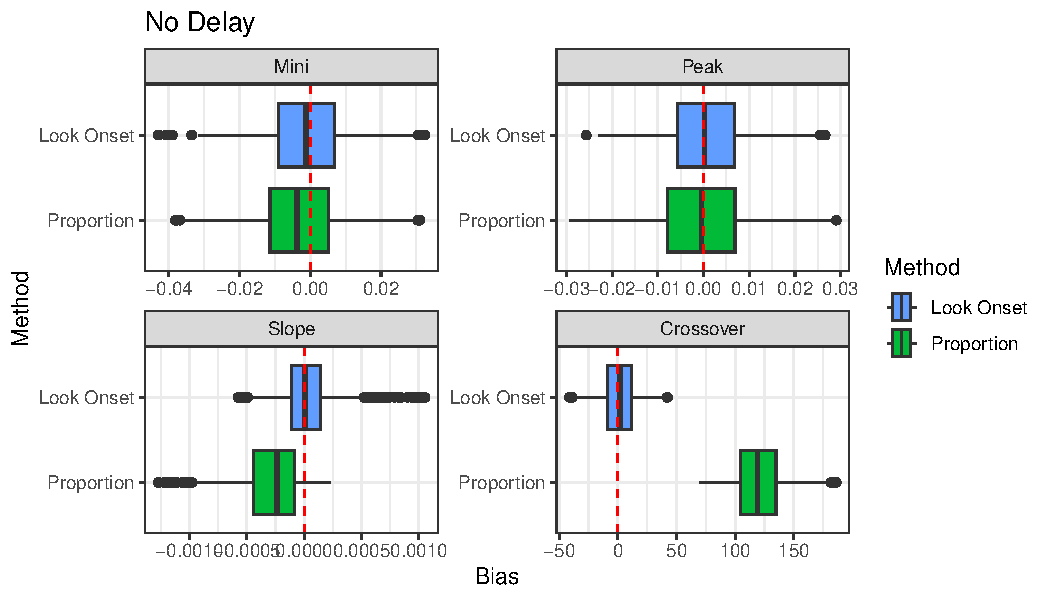
\includegraphics{no_delay_bar_plot.pdf}
\caption{Parameter bias with no oculomotor delay (x axis labels scrunched)}
\label{fig:par_bias_no_delay}
\end{figure}

\begin{figure}[H]
\centering
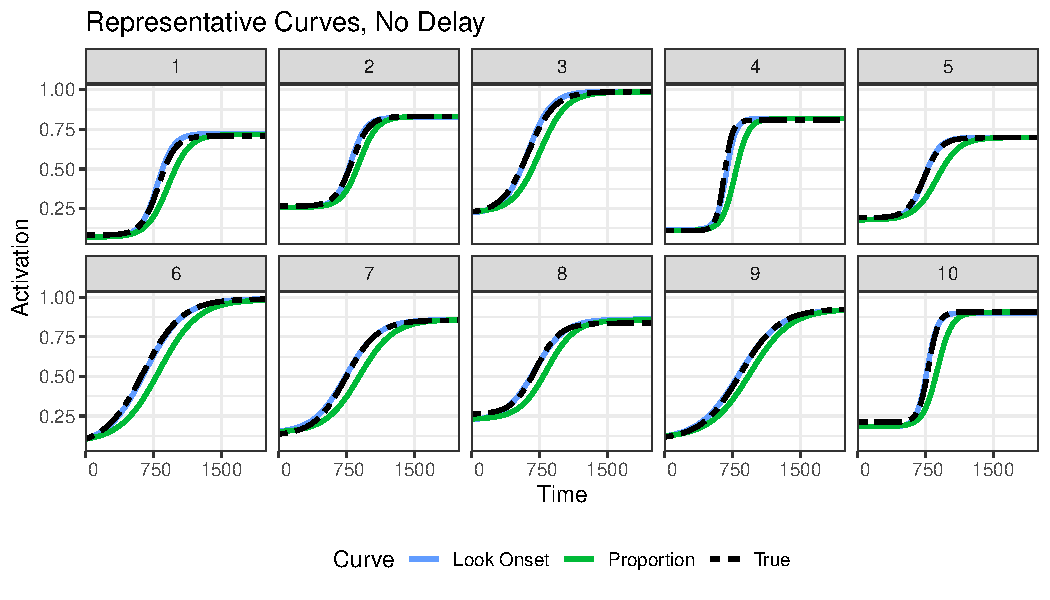
\includegraphics[width=0.9\textwidth]{rep_curves_no_delay.pdf}
\caption{Representative curves with no oculomotor delay}
\label{fig:rep_curves_no_delay}
\end{figure}
%
%
%
\subsection{Normal Delay}

\begin{figure}[H]
\centering
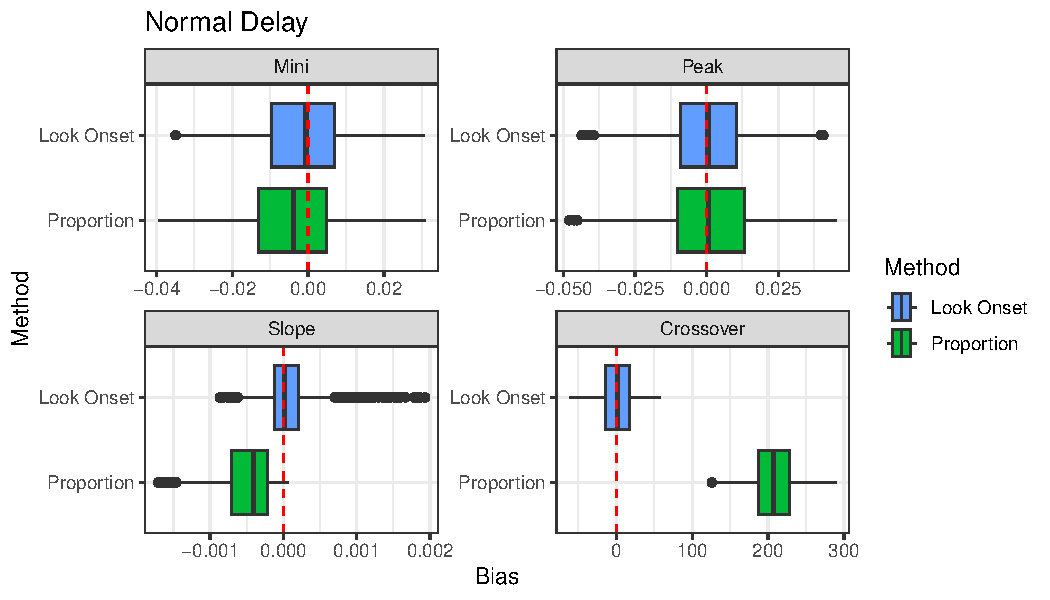
\includegraphics[scale=1]{normal_delay_bar_plot.pdf}
\caption{Parameter bias with normal oculomotor delay}
\label{fig:par_bias_normal_delay}
\end{figure}

\begin{figure}[H]
\centering
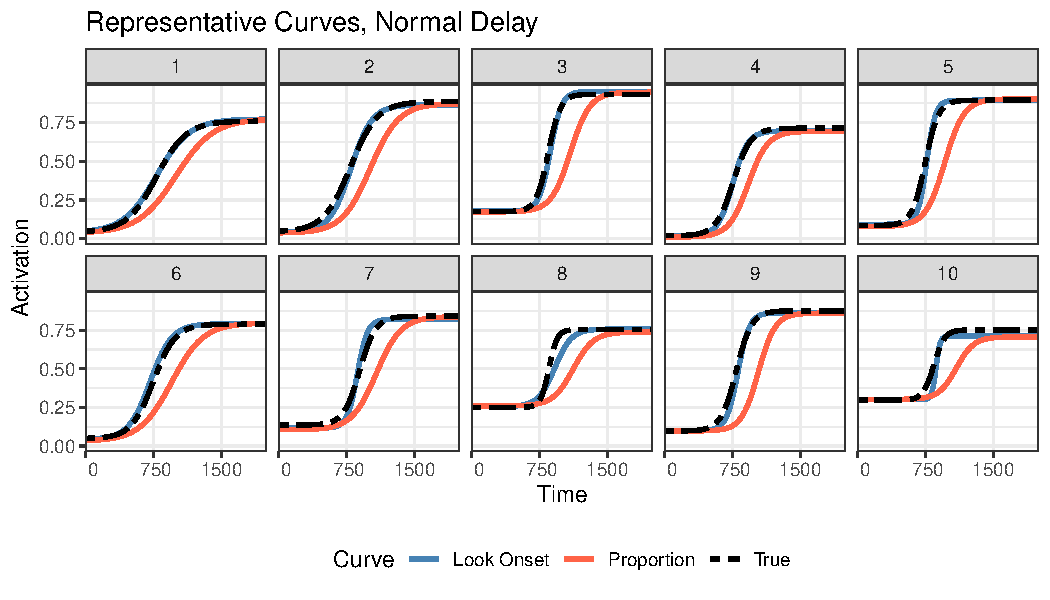
\includegraphics[width=0.9\textwidth]{rep_curves_normal_delay.pdf}
\caption{Representative curves with normal oculomotor delay}
\label{fig:rep_curves_normal_delay}
\end{figure}

\subsection{Weibull Delay}



\begin{figure}[H]
\centering
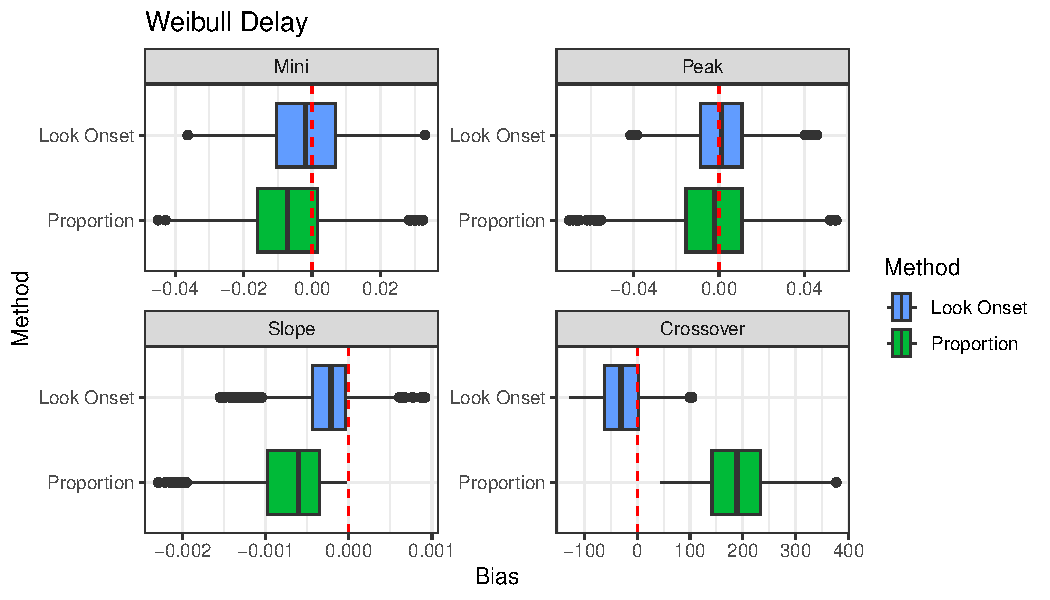
\includegraphics[scale=1]{weibull_delay_bar_plot.pdf}
\caption{Parameter bias with Weibull oculomotor delay}
\label{fig:par_bias_weibull_delay}
\end{figure}

\begin{figure}[H]
\centering
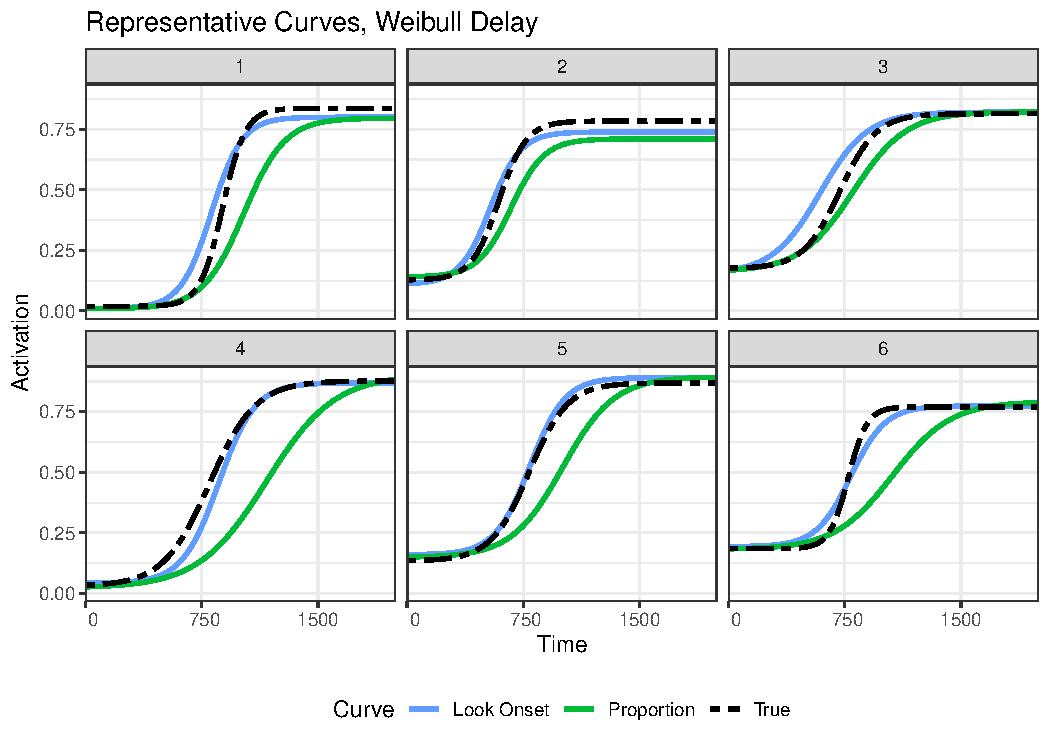
\includegraphics[width=0.9\textwidth]{rep_curves_weibull_delay.pdf}
\caption{Representative curves with Weibull oculomotor delay}
\label{fig:rep_curves_weibull_delay}
\end{figure}





\subsection{Results}

[I will go back and comment on results in each of the scenarios with broader discussion of implications in each, though normal and Weibull will be similar]

In addition to the visual summaries, we present in Table~\ref{tab:mise_sims} a summary of the mean integrated squared error (MISE) between the generating and recovered curves using each of the methods

We begin by noting the  magnitude of difference between the look onset method and the proportion of fixation method in the case of $\rho = 0$, or No Delay, demonstrating the amount of bias introduced in the proportion method. This alone demonstrates how critical of an issue the added observation bias is in the recovery of the underlying activation.

To assess the effects of randomness in the oculomotor delay, it seems prudent to limit the comparisons within each method. Considering first the look onset method, we see that as the degree of variability increases, so does the difficulty in correctly recovering the underlying curve. It is important to note that these magnitudes are meant to be relative rather than absolute: the particular values observed are a function of the relationship between the generating $\gamma$ distribution and that of $\rho$. Nonetheless, this does suggest a need to further investigate ways to control for the added uncertainty. To quickly comment on the apparently ``flipped" MISE for the proportion of fixation method as it relates to the normal and Weibull distributed oculomotor delay, it would seem as if the skew of the Weibull distribution acted in such a way as to actually offset some of the observed added observation bias and seems more an artifact of the simulation conditions rather than an inherent statement relating OM bias to the proportion of fixation method in general.

% latex table generated in R 4.2.2 by xtable 1.8-4 package
% Wed Feb  8 15:10:31 2023
\begin{table}[H]
\centering
\begin{tabular}{llrrr}
  \hline
Method & Delay & 1st Qu. & Median & 3rd Qu. \\ 
  \hline
Look Onset & No Delay & 0.17 & 0.32 & 0.56 \\ 
  Look Onset & Normal Delay & 0.37 & 0.71 & 1.24 \\ 
  Look Onset & Weibull Delay & 1.05 & 2.16 & 4.23 \\ 
  Proportion & No Delay & 8.21 & 11.33 & 16.01 \\ 
  Proportion & Normal Delay & 22.90 & 30.65 & 39.37 \\ 
  Proportion & Weibull Delay & 15.27 & 24.75 & 38.14 \\ 
   \hline
\end{tabular}
\caption{Summary of mean integrated squared error across simulations}
\label{tab:mise_sims}
\end{table}

The proportion of fixation method seems no longer tenable in the recovery the underlying lexical activation, given both the magnitude of differences presented in Table~\ref{tab:mise_sims} as well as the theoretical arguments made and illustrated in Figure~\ref{fig:folly_of_fixation}. And given that data collected via the look onset method can be adequately fit in the newest version of the \xt{bdots} software, there appears to be little to argue against its adoption.


\section{Discussion}

This section needs to be tightened quite a bit.

Through our investigation, we have presented a physiologically grounded model relating eye tracking data to underlying lexical access by placing emphasis singularly on the first instance of a look, discarding information on the rest of the look entirely. 

Of course, we know that longer fixations are relevant to the strength of consideration. One of the primary benefits of the proportion method is that it indirectly captures the duration of fixations, with longer times being associated with stronger activation. This is important when differentiating fixations associated with searching patterns (i.e., what images exist on screen?) against those associated with consideration (is this the image I've just heard?). However, implicit in the proportion of fixations method is a crucially overlooked assumption of a linear relationship between the fixation length and the activation. That is, insofar as the construction of the fixation curve is considered, a fixation persisting at 20ms after look onset (and well within the refraction period in which no new information regarding the cognitive mechanism or voluntary fixation could be obtained (see figure i haven't made yet)) is considered identical to a fixation persisting at 500ms after onset: both are undifferentiated in being recorded as either a $0$ or $1$. More likely it seems this would be more of an exponential relationship, with longer fixations offering increasingly more evidence of lexical activation. By separating the moment of onset from the look itself, we free ourselves to construct far more nuanced models. Put more succinctly, it is not that the look onset method considers the length of fixation irrelevant; rather, it makes no statement about it at all. How these mechanisms could be combined should be the focus of future research.

Another utility that comes to mind when considering the look onset method is how much sparser of a dataset is created. Consider, for example, fitting a mixed model to the four parameter logistic modeling individual trial data for each subject all together. Such models with proportion of fixation data typically infeasible with cumbersome autocorrelative structures found within a trial (from Bob's comment, need to find source). The present method, being a much sparser dataset, may be far more computationally tractable. 


The arguments presented here has hoped to satisfy two goals, agnostic to the linking hypothesis or functions ultimately decided upon. Foremost is the recognition that the mechanisms governing a look onset and the looks themselves follow separate mechanisms, and treating them as such requires fewer assumptions while still retaining the utility in fitting the same nonlinear curves to the observed data.

Second to this, we have put a name to two important sources of potential bias in the recovering of activation curves, generalizable beyond the particulars of the presented simulations. The first is the added observation bias, speaking again to the utility in separating the relevant mechanisms making up a look. And second is the delayed observation bias, bringing into focus the importance of reevaluating how we address bias and variability in the oculomotor delay.


In short, what we have hoped to accomplish here is not to drastically change the original assumptions presented in Allopenna (1996, but rather to qualify them in statistically sound ways. And really, that is pretty much it. Concluding sentence.


As a not really conclusion, I am sometimes left to wonder to what degree the proportion of fixation method was a  ``local minimum" in the pursuit of utilizing eye-tracking data. The proportion of fixations created an ostensible curve, prompting McMurray to establish theoretically grounded non-linear functions to model them. These, in turn, where shown to be suitable functions with which to model saccade data over a period of trials. Had saccades lent themselves so naturally to visualization as the proportion of fixations, perhaps that is where we may have started.


\section*{Appendices}

Omitting relation of this method to TRACE as it seems mostly unnecessary to the present argument 

\section{Misc OM Discussion}

[mainly exists to demonstrate that despite appearances, OM delay still worth further investigation]

Outside of a demonstration of its existence and potential consequence, little more has been said about addressing the delayed observation bias. Further, the consequences of the delayed observation (under the assumption that the mean value is correctly accounted for) seem almost trivial in comparison to the differences between it and the added observation bias. That being said, we believe there are still critical reasons for considering its significance.

As mentioned earlier, the particular values observed in these simulations are both a function of the relationship between the distribution generating $\gamma$ and that of $\rho$. However, they are also a function of the generating function itself. In particular, we draw attention to the degree of total variation $f$ over the interval $[a,b]$, defined as 

\begin{equation}
V(f) = \underset{\mathcal{P}}{\sup} \sum_{i=0}^{n_p-1} \left|f(t_{i+1} - f(t_i) \right|,
\end{equation}

where $\mathcal{P} = \{P = \{t_0, \dots, t_{n_p}\} \}$ is the set of all possible partitions of $[a,b]$. Despite appearances, this is a relatively straightforward metric in the case of monotone functions such as the logistic, where the total variation is simply $|f(b) - f(a)|$. To illustrate the relevance of this, consider a hypothetical situation in which the underlying activation we are wishing to recover is a constant function, $f(t) = c$, where the probability of fixating on a target is independent of time. In such a situation, a delayed observation would be of no issue; despite changes in time $t$, the probability $c$ remains unchanged. In contrast, consider a second hypothetical situation in which activation is defined exponentially, $f(t) = \exp(t)$. In this case, the impact of delayed observation depends drastically on time, when the delay in observation in the range of small values of $t$ have a drastically smaller impact than delayed observations when $t$ is large ($\exp(1) - \exp(0) = 1.7183$ while $\exp(11) - \exp(10) = 37848$, despite both cases having $\Delta t = 1$).

In short, these hypothetical situations detail how the magnitude of total variation can have differential effects on the delay in observation. Now consider again the logistic function in Figure~\ref{fig:logistic_definition} and imagine its domain partitioned into three equally sized portions. Both the first and third, near the asymptotes, have relatively low total variation, resulting in a relatively benign effect from oculomotor delay. In contrast, the middle third contains nearly all of the variation of the function, indicating the delayed observation here will have a disproportionate impact on the successful recovery of the function. Given the clinical relevance of the both the slope and crossover parameters, as well as acknowledging the impact that these have on the overall shape of the function, we demonstrate a need in a accounting for this delay precisely where it will impact function recovery the most. This, of course, is not unique to the logistic, with the effects of the delayed observation bias compounded in the asymmetric Gaussian functions (appendix) which has a more complicated variation structure and, accordingly, more difficulty in recovering the generating curves.


%\section{Recovery of Individual Curves -- Asymmetric Gaussian}

Presented here are the results of the simulations for the recovery of subject-specific curves generated with the asymmetric Gaussian function, the parametric function typically associated with looks to competitors in the VWP. As in the section fitted with the logistic function, simulations include settings in which there is no oculomotor delay, as well as delay that is normally and Weibull distributed. Again, as all fits could not be individual examined, an automated criterion was used to determine which fits were considered  adequate. Here, this stipulated that the estimated sigma parameters be positive and that the height parameter be larger than either of the base parameters. The number of fits retained for the no delay, normal delay, and Weibull delay were  855, 786, and 816, respectively.


\subsection{Results}

As might be expected, the more complicated mean structure provided by the asymmetric Gaussian led to a generalized increase in the difficulty of recovery for both the look onset and proportion methods, relative to those generated with a logistic mean structure. However, we do still find that in the case of no delay, given in Figure~\ref{fig:dg_rep_curves_no_delay}, that the recovery of individual parameters is still unbiased and, as with the logistic, the location parameter (here, mu), is right shifted.

The results for the median integrated squared error are given in Table~\ref{tab:dg_mise_sims}. We again see results similar to those with the logistic in that the look onset method outperforms the proportion of fixation method in all cases. 

\begin{figure}[H]
\centering
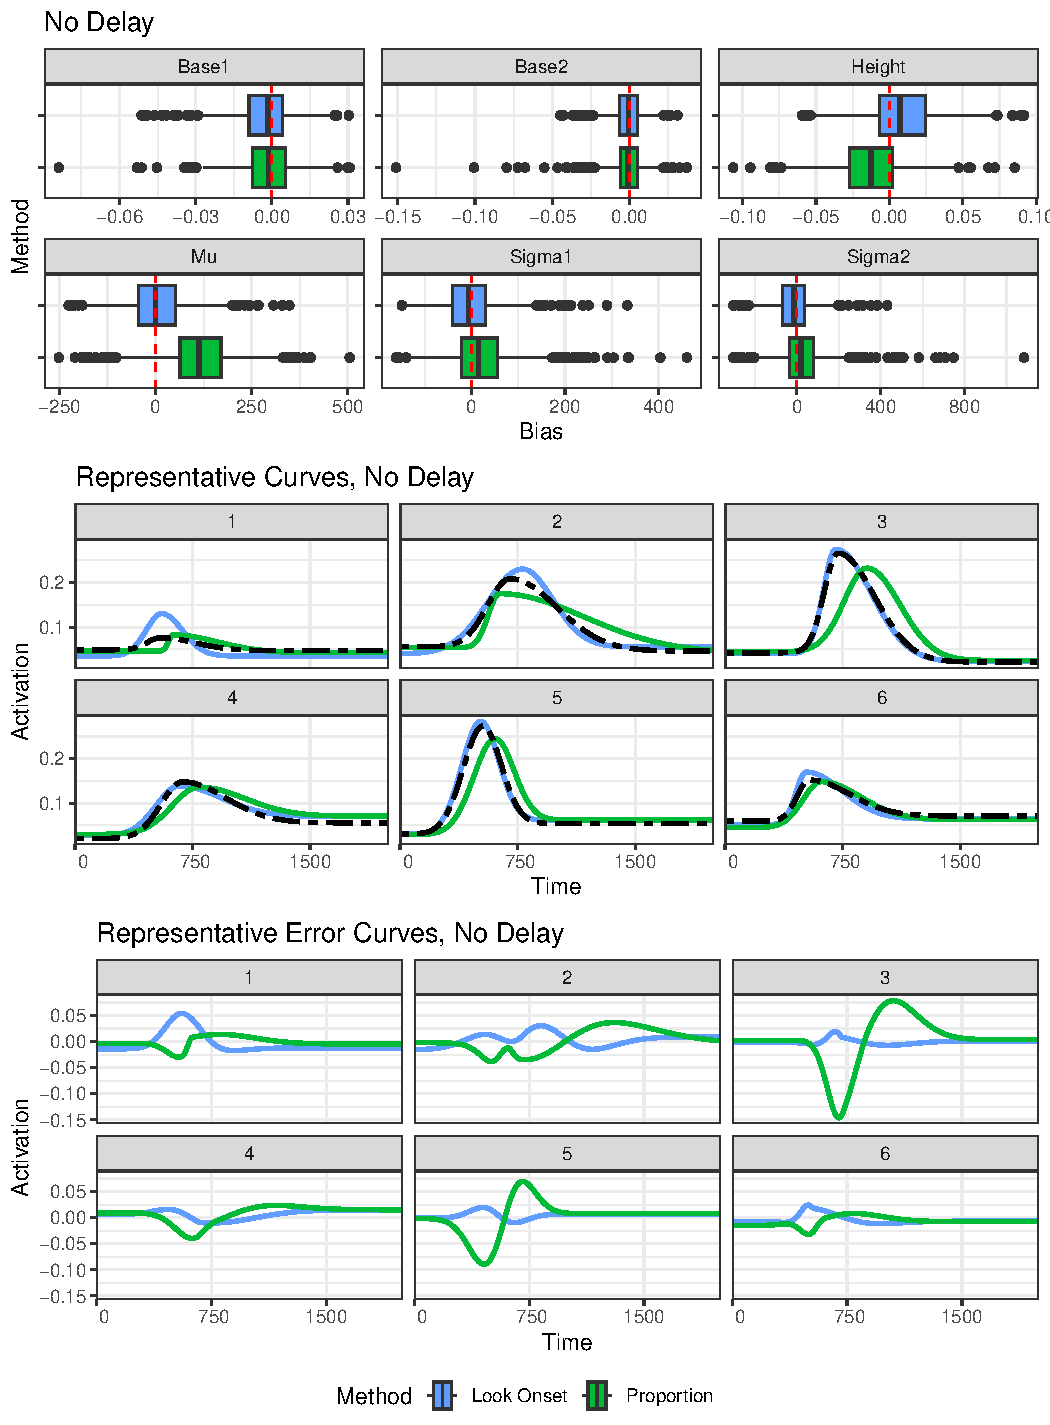
\includegraphics[width=0.9\textwidth]{dg_rep_and_diff_no_delay.pdf}
\caption{Summary of simulation results in the recovery of subject-specific curves generated by the asymmetric Gaussian with no oculomotor delay}
\label{fig:dg_rep_curves_no_delay}
\end{figure}

\begin{figure}[H]
\centering
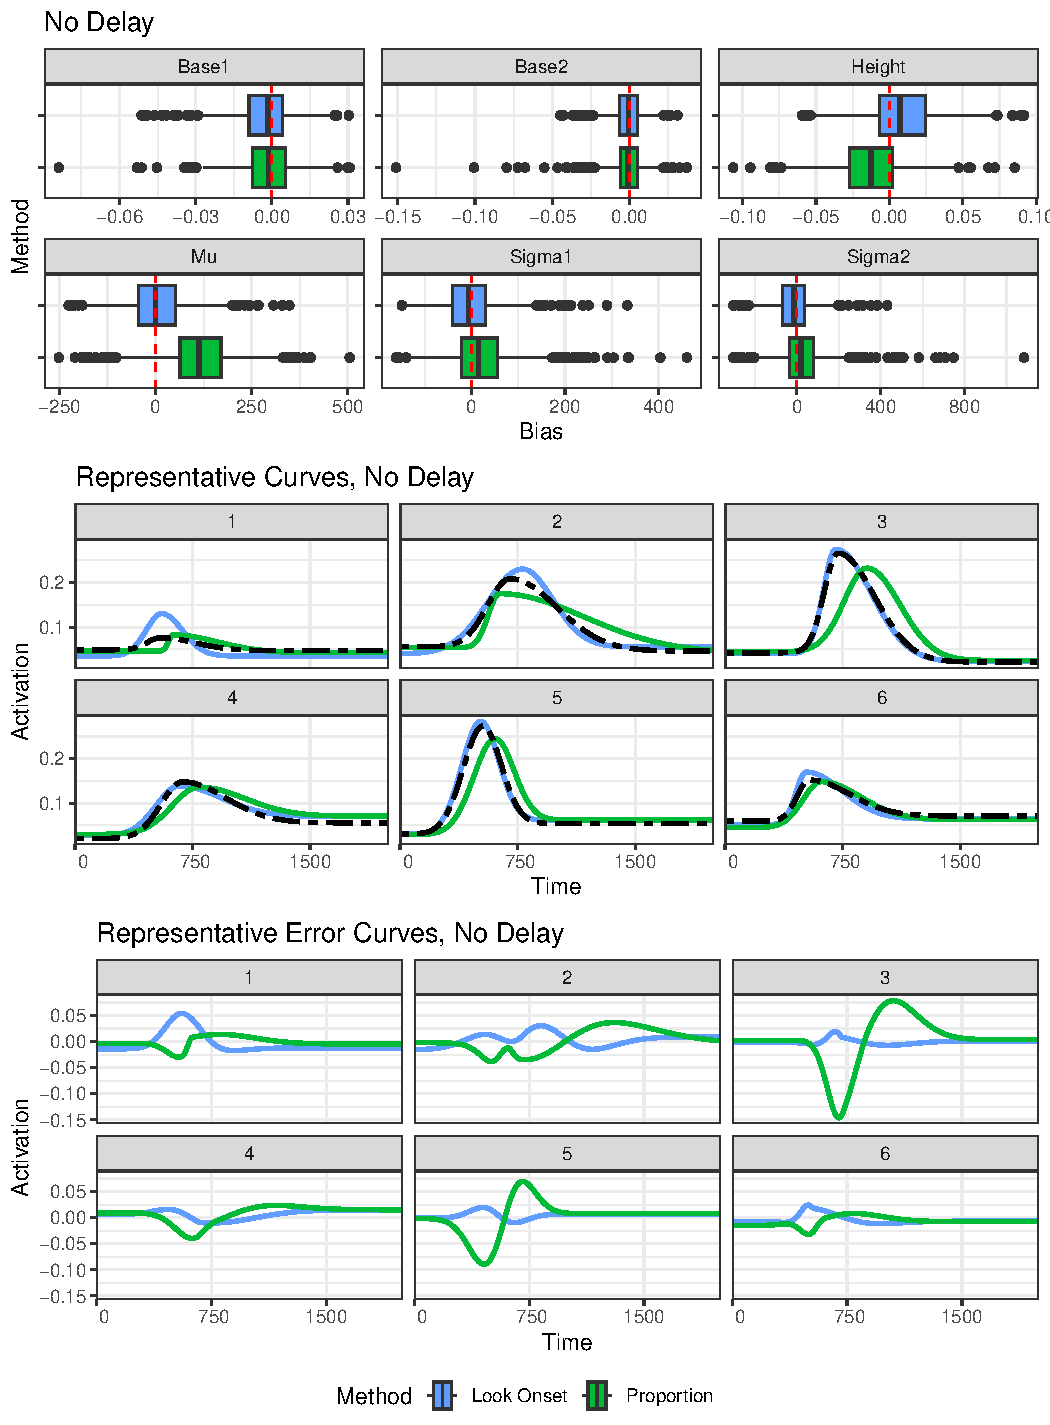
\includegraphics[width=0.9\textwidth]{dg_rep_and_diff_no_delay.pdf}
\caption{Summary of simulation results in the recovery of subject-specific curves generated by the asymmetric Gaussian with normally distributed oculomotor delay}
\label{fig:dg_rep_curves_normal_delay}
\end{figure}


\begin{figure}[H]
\centering
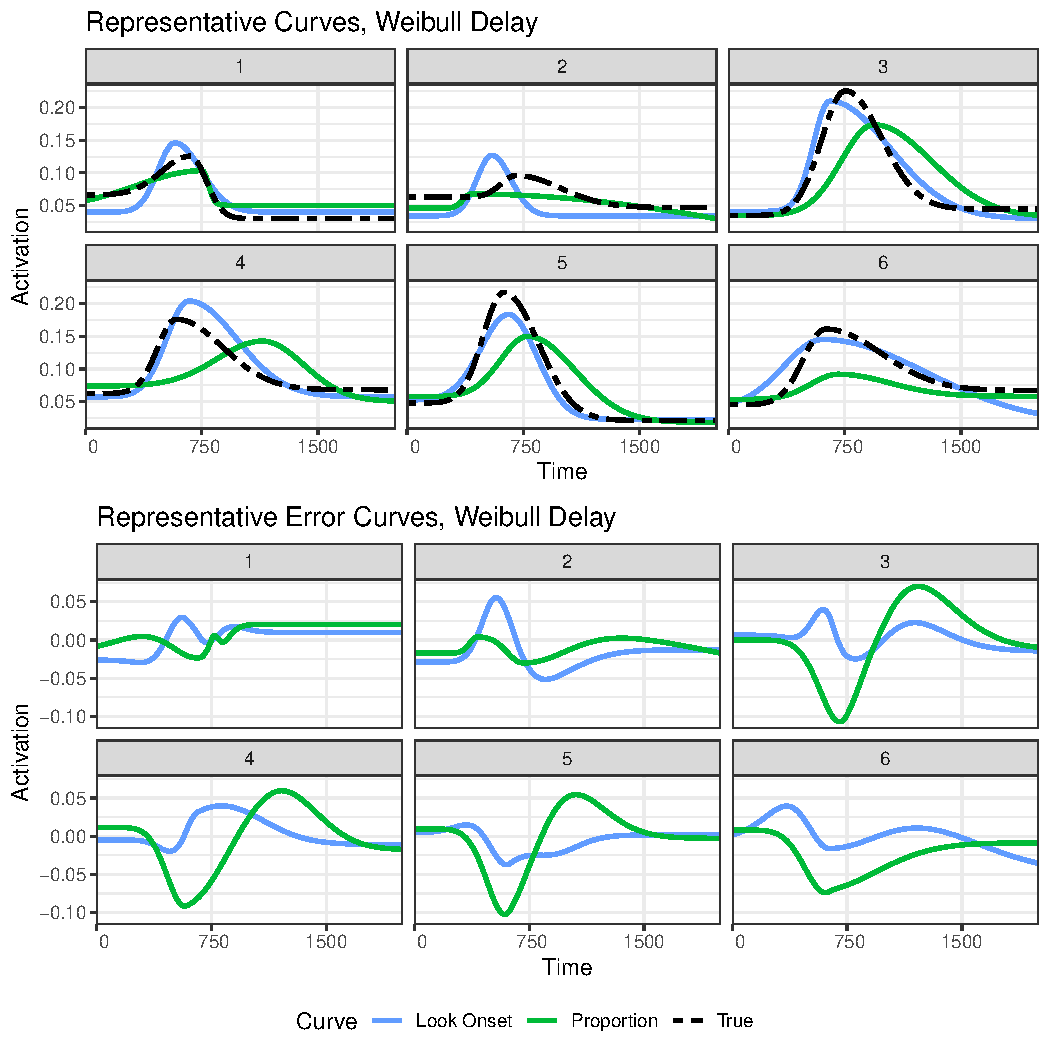
\includegraphics[width=0.9\textwidth]{dg_rep_and_diff_weibull_delay.pdf}
\caption{Summary of simulation results in the recovery of subject-specific curves generated by the asymmetric Gaussian with Weibull distributed oculomotor delay}
\label{fig:dg_rep_curves_weibull_delay}
\end{figure}




\begin{table}[H]
\centering
\begin{tabular}{llrrr}
  \hline
Curve & Delay & 1st Qu. & Median & 3rd Qu. \\ 
  \hline
Look Onset & No Delay & 0.22 & 0.36 & 0.63 \\ 
  Look Onset & Normal Delay & 0.38 & 0.70 & 1.15 \\ 
  Look Onset & Weibull Delay & 0.52 & 0.84 & 1.39 \\ 
  Proportion & No Delay & 0.75 & 1.29 & 2.08 \\ 
  Proportion & Normal Delay & 1.38 & 2.44 & 3.96 \\ 
  Proportion & Weibull Delay & 1.00 & 1.98 & 3.43 \\ 
   \hline
\end{tabular}
\caption{Median integrated squared error for recovery of individual curves generated with asymmetric Gaussian}
\label{tab:dg_mise_sims}
\end{table}

\subsection{$R^2$ for Recovery of Individual Curves}

Here, we provide an alternative summary of the recovery of subject specific curves fit with both the logistic and asymmetric Gauss. 


\subsubsection{Logistic}

\begin{table}[H]
\centering
\begin{tabular}{llrrr}
  \hline
Curve & Delay & 1st Qu. & Median & 3rd Qu. \\ 
  \hline
Look Onset & No Delay & 1.00 & 1.00 & 1.00 \\ 
  Look Onset & Normal Delay & 0.99 & 1.00 & 1.00 \\ 
  Look Onset & Weibull Delay & 0.98 & 0.99 & 0.99 \\ 
  Proportion & No Delay & 0.92 & 0.94 & 0.95 \\ 
  Proportion & Normal Delay & 0.80 & 0.83 & 0.86 \\ 
  Proportion & Weibull Delay & 0.80 & 0.86 & 0.91 \\ 
   \hline
\end{tabular}
\caption{$R^2$ for Logistic}
\label{tab:r2_logistic_sims}
\end{table}

\subsubsection{Asymmetric Gaussian}

\begin{table}[H]
\centering
\begin{tabular}{llrrr}
  \hline
Curve & Delay & 1st Qu. & Median & 3rd Qu. \\ 
  \hline
Look Onset & No Delay & 0.80 & 0.91 & 0.95 \\ 
  Look Onset & Normal Delay & 0.63 & 0.82 & 0.91 \\ 
  Look Onset & Weibull Delay & 0.57 & 0.77 & 0.87 \\ 
  Proportion & No Delay & 0.48 & 0.65 & 0.75 \\ 
  Proportion & Normal Delay & 0.10 & 0.33 & 0.52 \\ 
  Proportion & Weibull Delay & 0.20 & 0.46 & 0.64 \\ 
   \hline
\end{tabular}
\caption{$R^2$ for Asymmetric Gaussian}
\label{tab:r2_dg_sims}
\end{table}



\section{IRL data}

This needs to be moved but then a lot of this document needs restructuring. At any rate, here is what we have. We use the dataset collected in \cite{mcmurray2010individual} which measured eye tracking in cohort of adolescents including 40 typically developed (N), 16 specific cognitive impaired (SCI), 20 specific language impaired (SLI), and 17 non-specific language impaired. They did a standard vwp trial and here are the details [...]. While this study predates the \xt{bdots} software,  we can go back and assess these groups doing a typical analysis.  In doing so, we did a factorial comparison of all pairwise groups, resulting in 6 total comparisons. We did this with both look onset transformed data, as well as standard proportion of fixation data. Of the six comparisons made, only two were found to have significant differences between group curves, in the comparison of CF/NLI and N/NLI. Further, these differences were only identified with the look onset method. That is, for all six comparisons, the proprotion of fixation methods failed to identify any curves that were different between groups.

Should talk about the reasonable transformation I did to arrive at look onset data

\begin{figure}[H]
    \centering
    \subfigure[]{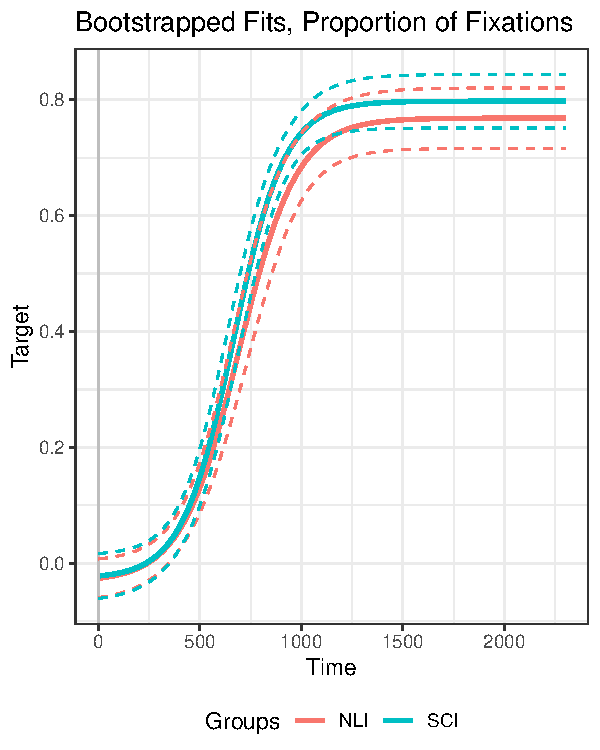
\includegraphics[width=0.45\textwidth]{irl_data_prop_1}}
    \subfigure[]{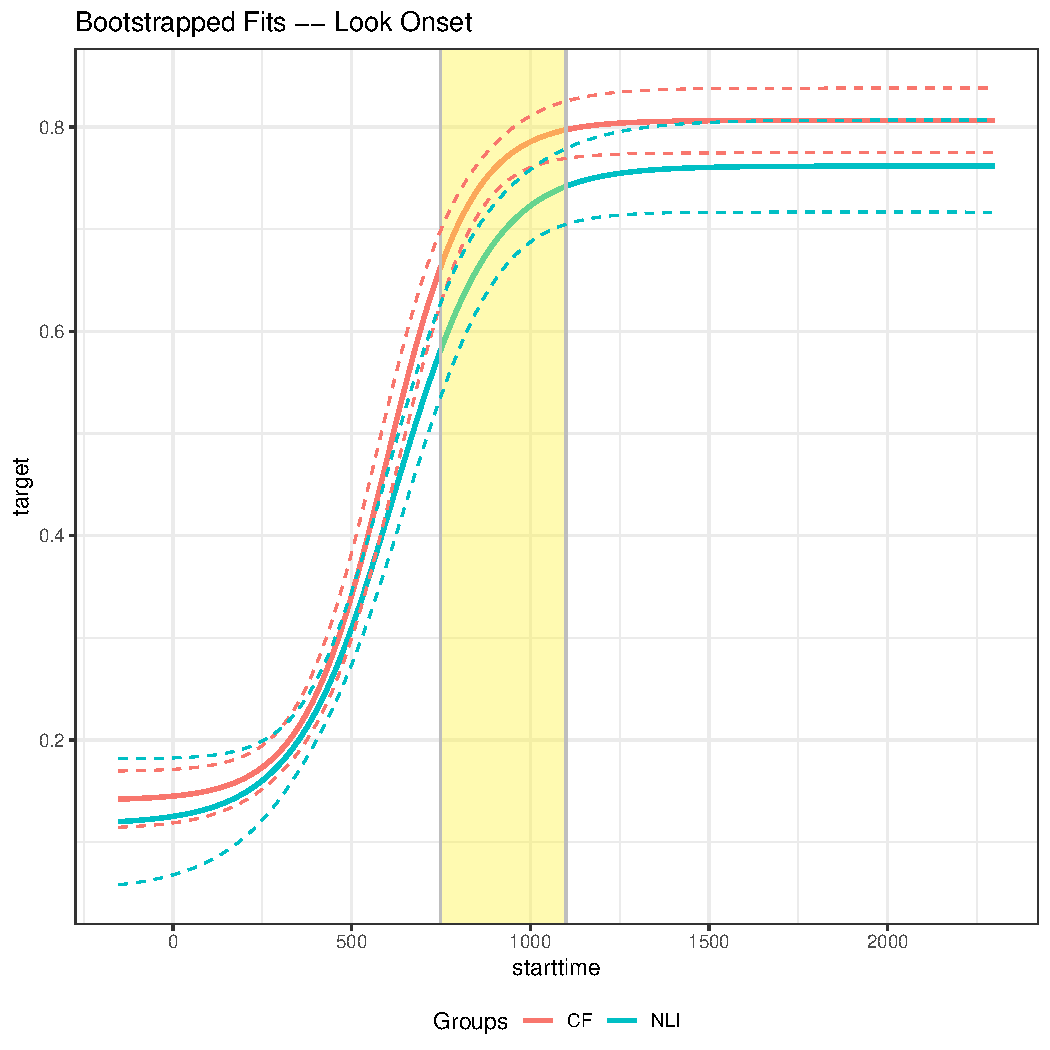
\includegraphics[width=0.45\textwidth]{img/irl_data_onset_1}}
    \caption{(a) is proportion of fixations, (b) is look onset. This is comparing CF vs NLI}
\label{fig:irldata1}
\end{figure}

\begin{figure}[H]
    \centering
    \subfigure[]{
\includegraphics[width=0.45\textwidth]{irl_data_prop_2}}
    \subfigure[]{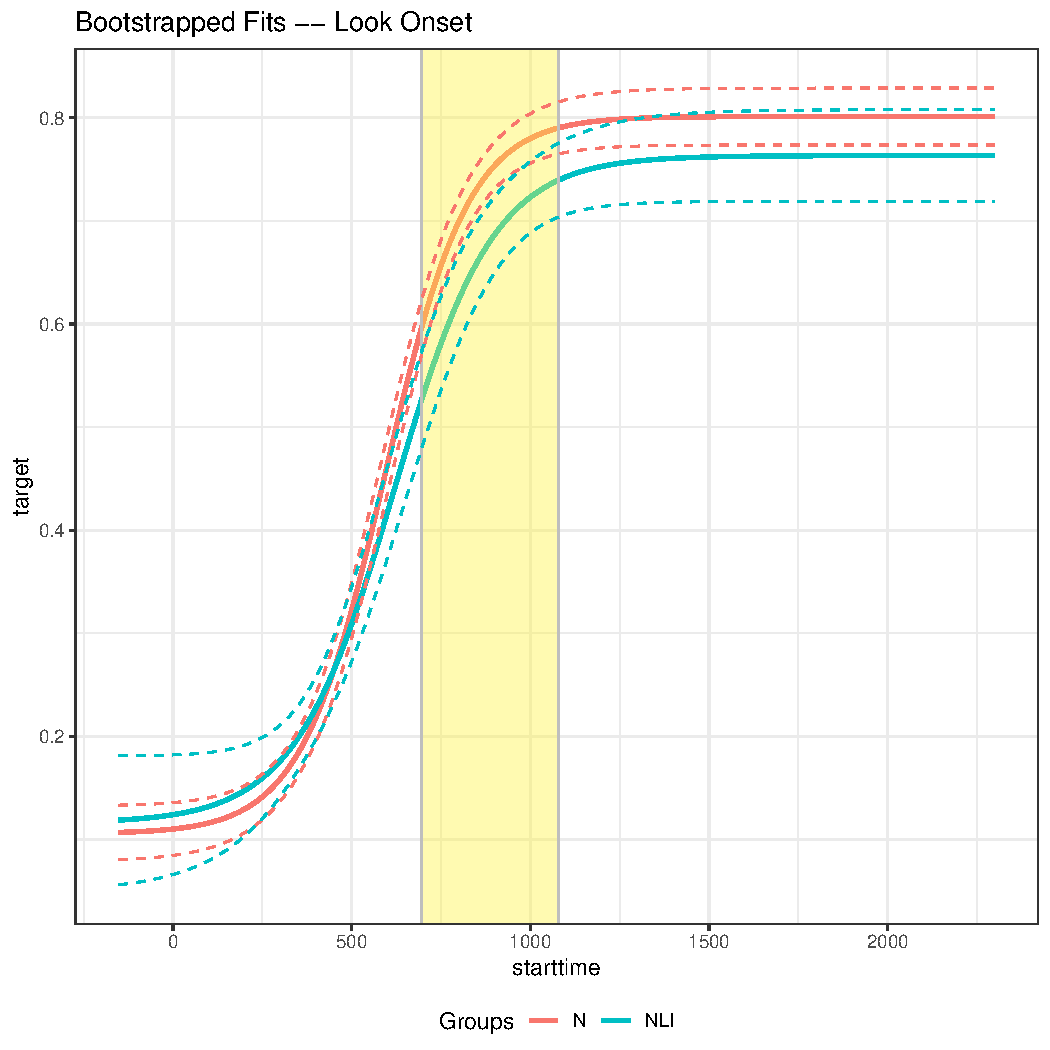
\includegraphics[width=0.45\textwidth]{img/irl_data_onset_2}}
    \caption{(a) is proportion of fixations, (b) is look onset. This is comparing N vs NLI}
\label{fig:irldata2}
\end{figure}




